\section{Risco Aplicado ao Setor Elétrico}

\subsection{Introdução}
  No contexto, apresentado nas aulas anteriores com relação a incerteza no setor elétrico, nesta aula será apresentado o conceito de medida de risco e suas aplicações. Assim, esta aula tem como objetivo gerir o risco nos contratos e como contratar de maneira ótima.
  Inicialmente a medida de risco pode ser definida com a tentativa de medir o grau de incerteza na obtenção do retorno esperado em alguma aplicação financeiro ou investimento realizado. Assim, elas buscam atacar o problema “risco” de resultados indesejáveis de forma mais direta e pragmática, onde a distribuição dos valores financeiros seriam diretamente monitoradas e “controladas” através destas medidas e de valores limites de exposição (que podem ser estipulados a priori pelos agentes). 
  Os agentes podem se comportar de maneiras diferentes diferentes em relação ao risco podendo ser avesso, neutro ou propenso. O agente avesso ao risco é aquele que o valor da perda é mais importante no critério de decisão do que valor de um ganho futuro, ou seja este agente está interessado nem risco de perda menores. O agente neutro ao risco é o investidor indiferente ao risco,onde o ganho possui o mesmo impacto que a perda de uma loteria.E por fim um agente propenso ao risco se importa mais com os ganhos do que com as perdas que a loteria vai retornar, ao contrário do investidor avesso ao risco. A figura \ref{fig:aula10_1_1} representa o comportamento do perfil de risco do agente.
 
\begin{figure}[H]
\begin{centering}
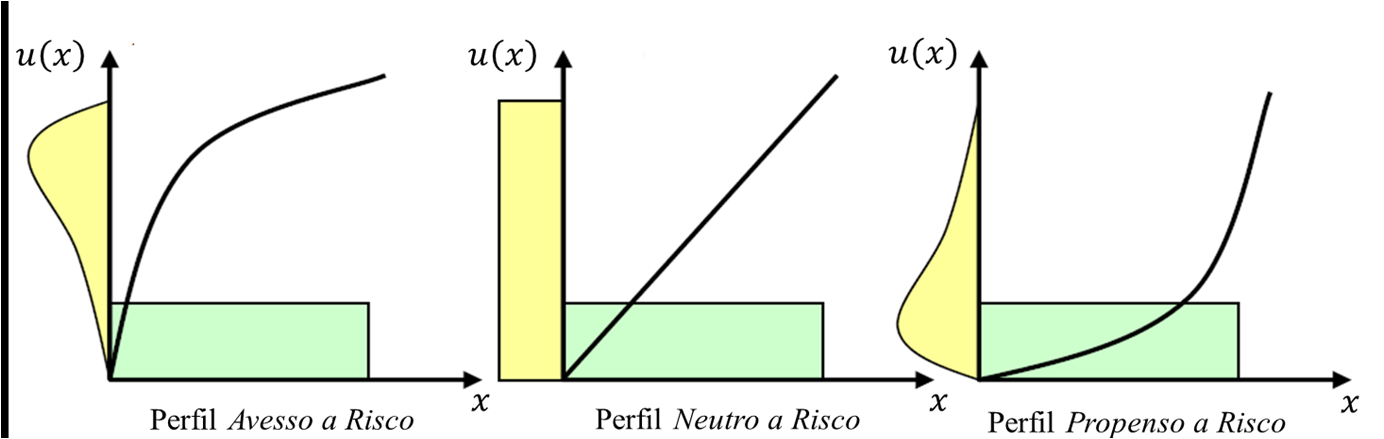
\includegraphics[scale=0.6]{aula10_1_1}\protect\caption{\label{fig:aula10_1_1} Perfil do agente}
\end{centering}
\end{figure}

O para utilizar o risco nesta aula usaremos o modelo probabilístico para a construção do problema. Assim,para utilizarmos o conceito de risco, é necessário o uso de variáveis aleatórias: \[
\tilde{X}(\omega):\Omega\rightarrow\mathbb{R}
\]
Onde,$\Omega$ é o conjunto de cenários,ou seja,possíveis estados da natureza. No caso discreto $\Omega_{N}$ é finito e enumerável  e contem $N$ elementos, representado por,
\[
\{X_{\omega},p_{\omega}\}_{\omega\in\Omega}.
\]
 Variáveis aleatórias são funções que ligam um cenário dentro do espaço amostral a um número real. Para abordar de maneira clara o conceito de variável aleatória suponha um caso discreto, $\Omega_{5}=\{1,...,5\}$ e as possíveis variáveis aleatórias associadas as suas probabilidades representadas por:
 \[
\{\pi_{\omega},p_{\omega}\}_{\omega\in\Omega_{5}}.
\]

Temos,

\begin{tabular}{|c|c|}
\hline 
$\pi$ & Probabilidade\tabularnewline
\hline 
\hline 
10 & 0,1\tabularnewline
\hline 
50 & 0,2\tabularnewline
\hline 
100 & 0,4\tabularnewline
\hline 
200 & 0,2\tabularnewline
\hline 
400 & 0,1\tabularnewline
\hline 
\end{tabular}

 Outro conceito importante para a introdução da medida de risco é função de distribuição de probabilidade acumulada($F_{\tilde{\pi}}(\pi)=P(\tilde{\pi}\leq\pi)$), onde pode ser representada em um caso discreto na figura \ref{fig:aula10_1}. Onde é construída com base na função densidade de probabilidade($f_{\tilde{\pi}}(\pi)=\frac{\partial F_{\tilde{\pi}}}{\partial\pi}\cdot(\pi)$) representada de forma gráfica na figura \ref{fig:aula10_2}.

\begin{figure}[H]
\begin{centering}
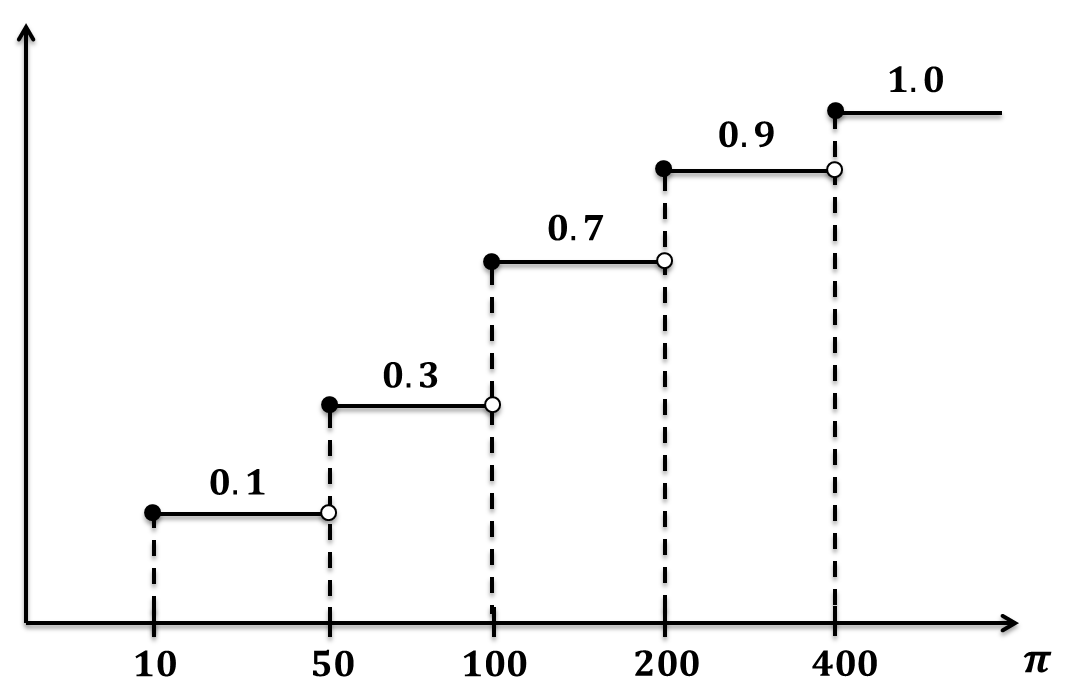
\includegraphics[scale=0.6]{aula10_1}\protect\caption{\label{fig:aula10_1} Função acumulada da variável aleatória discreta}
\end{centering}
\end{figure}

\begin{figure}[H]
\begin{centering}
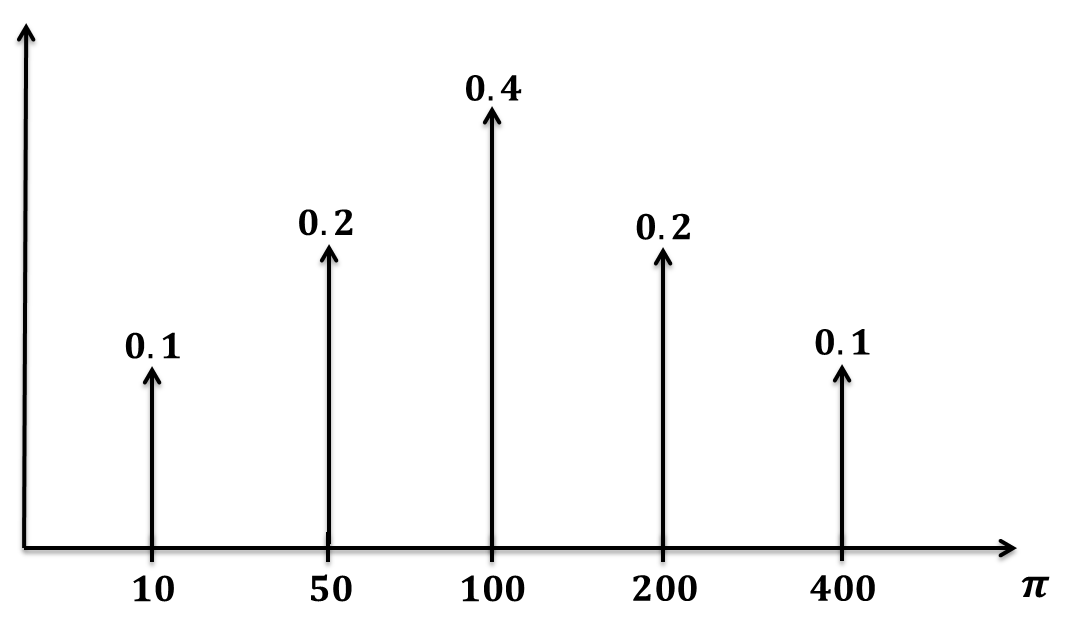
\includegraphics[scale=0.6]{aula10_2}\protect\caption{\label{fig:aula10_2} Densidade de probabilidade discreta}
\end{centering}
\end{figure}

 Para variáveis aleatórias contínuas ,como a normal, a função de probabilidade acumulada (\ref{fig:aula10_3}) e função densidade de probabilidade (\ref{fig:aula10_4}) são representadas com diferentes médias e desvios.
\begin{figure}[H]
\begin{centering}
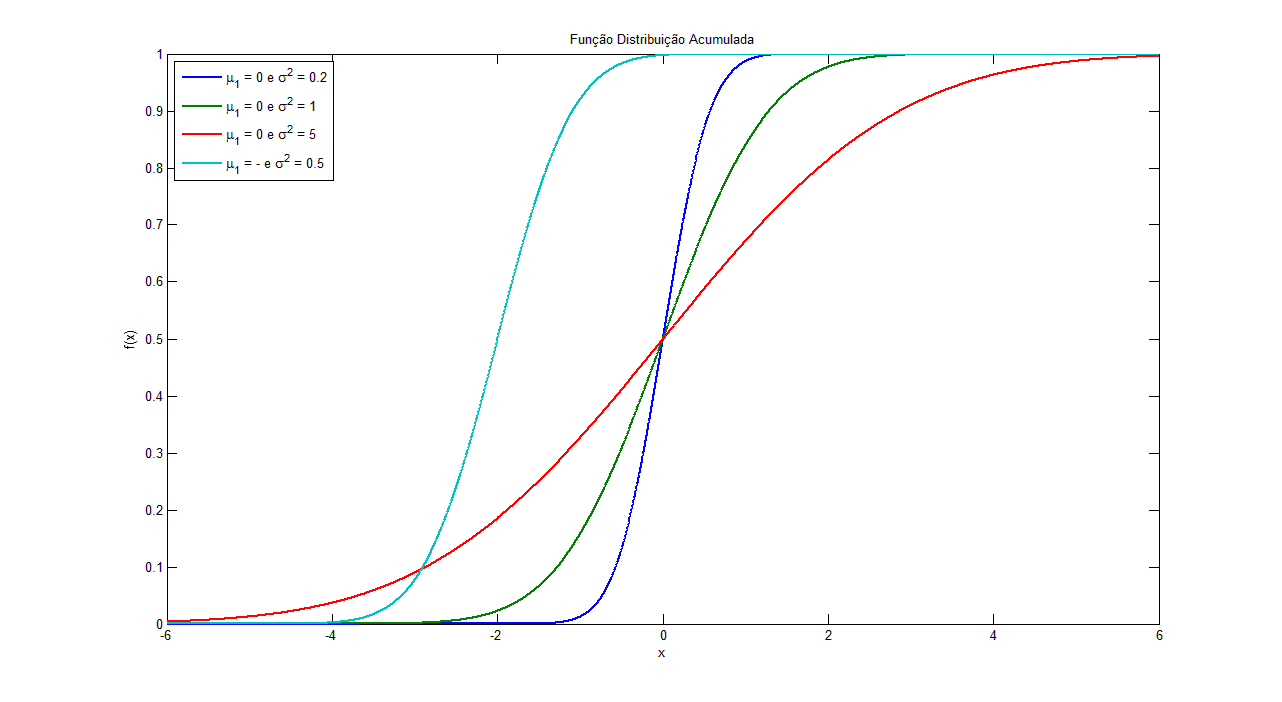
\includegraphics[scale=0.4]{aula10_3}\protect\caption{\label{fig:aula10_3} Função acumulada da variável aleatória contínua}
\end{centering}
\end{figure}

\begin{figure}[H]
\begin{centering}
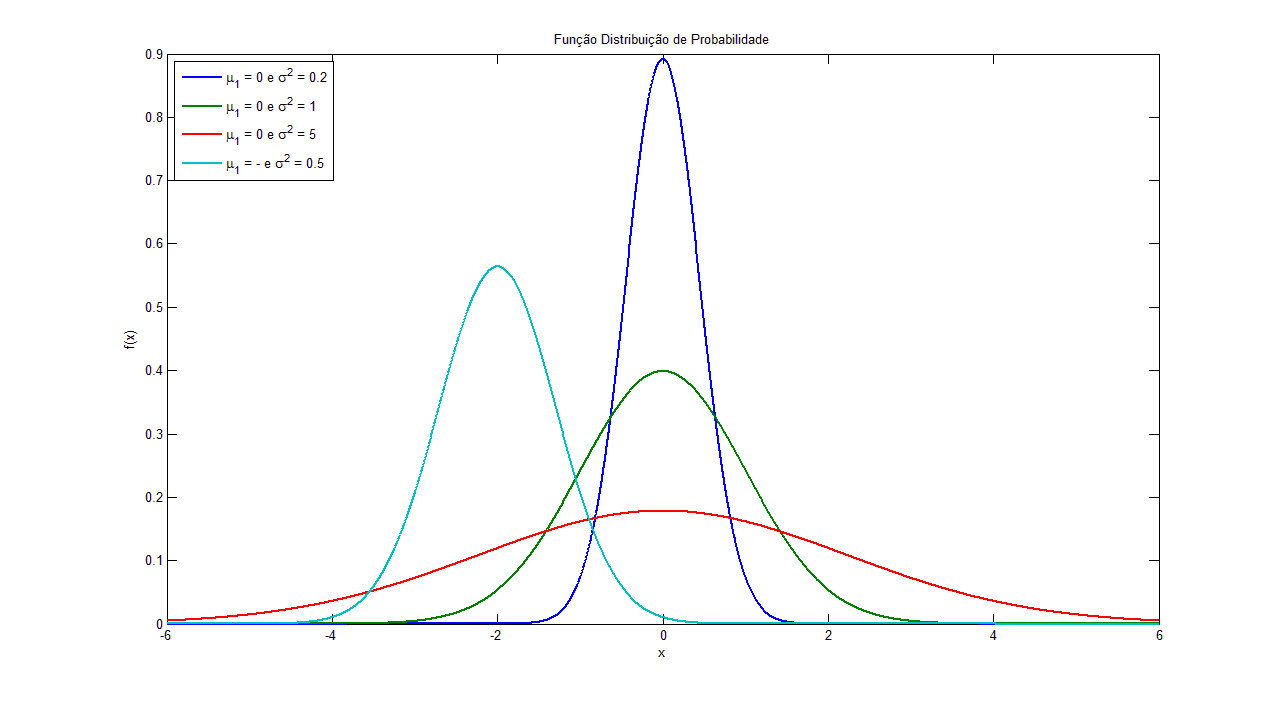
\includegraphics[scale=0.4]{aula10_4}\protect\caption{\label{fig:aula10_4} Densidade de probabilidade contínua}
\end{centering}
\end{figure}

 Para facilitar os cálculos abordaremos o uso da variável aleatória discreta, poderemos aproximar uma distribuição de probabilidade contínua para uma distribuição de probabilidade discreta através de simulações de Monte Carlo.
 
\subsection{Simulação}

 A simulação tem como objetivo replicar o comportamento de sistemas complexos explorando a aleatoriedade dos eventos acontecerem, para isso é necessário a obtenção de cenários das possíveis saídas do sistema. E devida a esta aleatoriedade os métodos de simulação são conhecidos como métodos de Monte Carlo, este nome é referente ao cassino de Mônaco e se tornou popular pelos pesquisadores Stanislaw Ulam, Enrico Fermi, John von Neumann e Nicholas Metropolis.
 Então é possível representar (aproximadamente) uma distribuição a partir de uma simulação Monte Carlo (sorteio ou amostragem aleatória) simulando ou amostrando um conjunto de $N$ valores da variável aleatória de maneira independente e atribuindo a cada um desses cenários a mesma probabilidade igual a $\frac{1}{N+1}$. Após esta realização teremos uma distribuição de probabilidade discreta com $N$ possíveis valores com probabilidade  $\frac{1}{N+1}$, esta variável aleatória é necessária para montar a função acumulada. Suponha que sorteamos três números aleatórios, isso significa que discretizamos o espaço amostral em quatro, apresentado na figura\ref{fig:aula10_5}.
 

\begin{figure}[H]
\begin{centering}
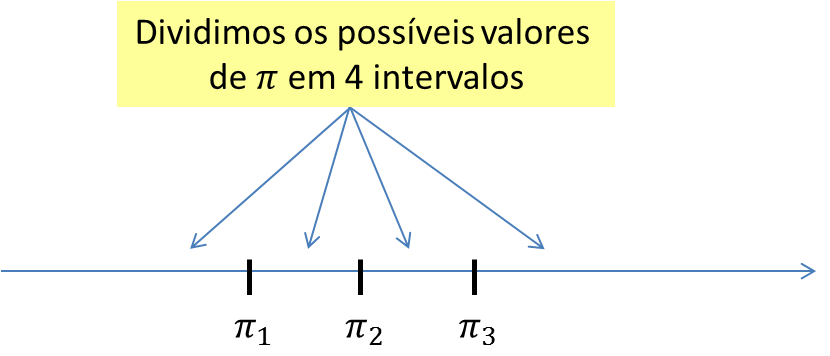
\includegraphics[scale=0.6]{aula10_5}\protect\caption{\label{fig:aula10_5} Simulação de Monte Carlos}
\end{centering}
\end{figure}
 Um ponto importante que pode ser questionável é como podemos simular variáveis equiprováveis aproximam distribuições com probabilidades diferentes, a justificativa é que, com a simulação de muitos cenários de uma variável aleatória com determinada distribuição, haverá uma concentração maior de realizações em torno dos valores com maior probabilidade de ocorrência (figura \ref{fig:aula10_7})

\begin{figure}[H]
\begin{centering}
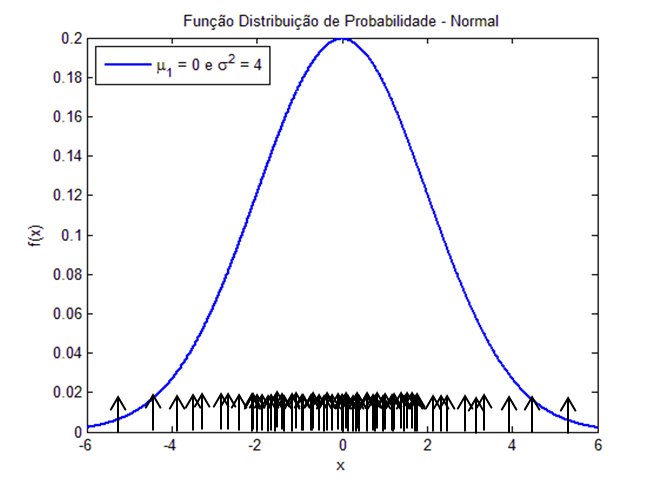
\includegraphics[scale=0.6]{aula10_7}\protect\caption{\label{fig:aula10_7} Simulação aproximada da fdp}
\end{centering}
\end{figure}

 Assim, soma das probabilidades, $\frac{1}{N+1}$, dentro de intervalos especificados converge para a probabilidade teórica da variável aleatória simulada dentro deste mesmo intervalo (figura \ref{fig:aula10_8}).

\begin{figure}[H]
\begin{centering}
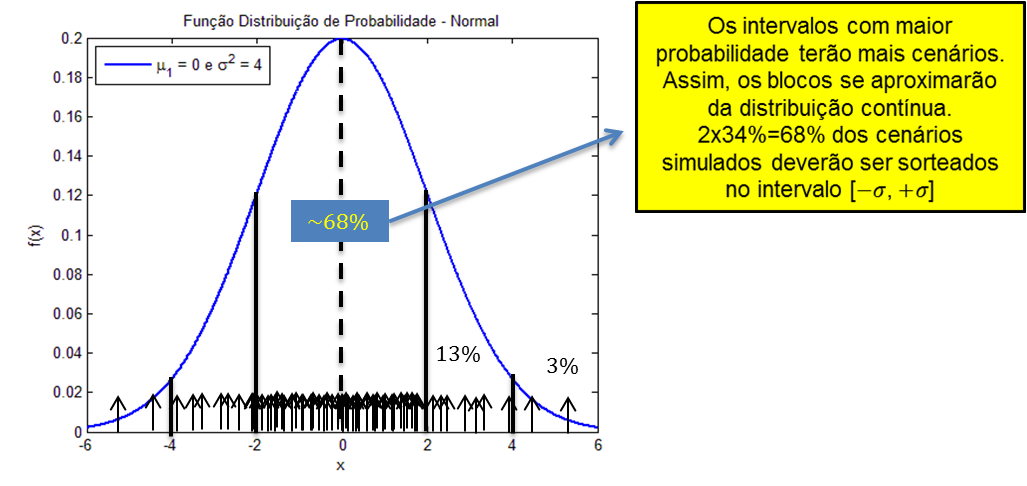
\includegraphics[scale=0.6]{aula10_8}\protect\caption{\label{fig:aula10_8} Simulação aproximada da função densidade de probabilidade dentro de intervalos}
\end{centering}
\end{figure}

 Quando $N\rightarrow\infty$, a curva de distribuição acumulada da distribuição produzida pela simulação converge para a da variável aleatória utilizada para a simular simular os dados e a distribuição acumulada pode ser obtida ordenando os valores simulados (figura \ref{fig:aula10_9}).

\begin{figure}[H]
\begin{centering}
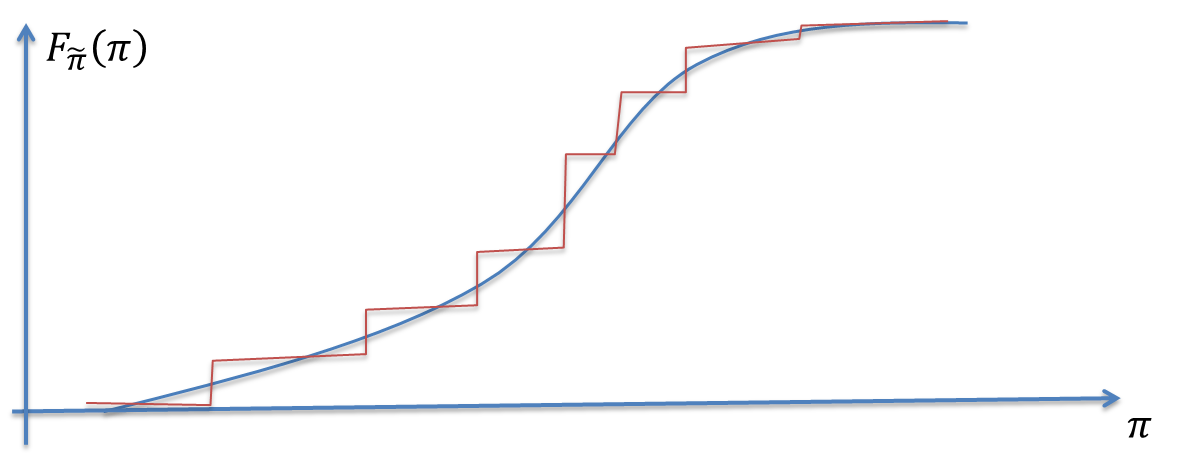
\includegraphics[scale=0.6]{aula10_9}\protect\caption{\label{fig:aula10_9} Simulação aproximada da função densidade de probabilidade dentro de intervalos}
\end{centering}
\end{figure}

Por exemplo podemos simular uma Normal(0,1), com 5 cenários (figura\ref{fig:aula10_10}), com 50 cenários (figura\ref{fig:aula10_11}), com 200 cenários (figura\ref{fig:aula10_12}) e com 2000 cenários (figura\ref{fig:aula10_13}). Assim podemos perceber através das figuras que quanto maior o número de cenários ocorrerá a aproximação da simulação com a distribuição de probabilidade teórica.
Conclui-se então que simulando um grande número de cenários, a distribuição de
probabilidade de todas as saídas da simulação de variáveis aleatórias discretas podem ser aproximados com precisão uma distribuição de probabilidade de variáveis aleatórias contínuas e essa precisão aumenta à medida que o número de cenários aumentam.

\begin{figure}[H]
\begin{centering}
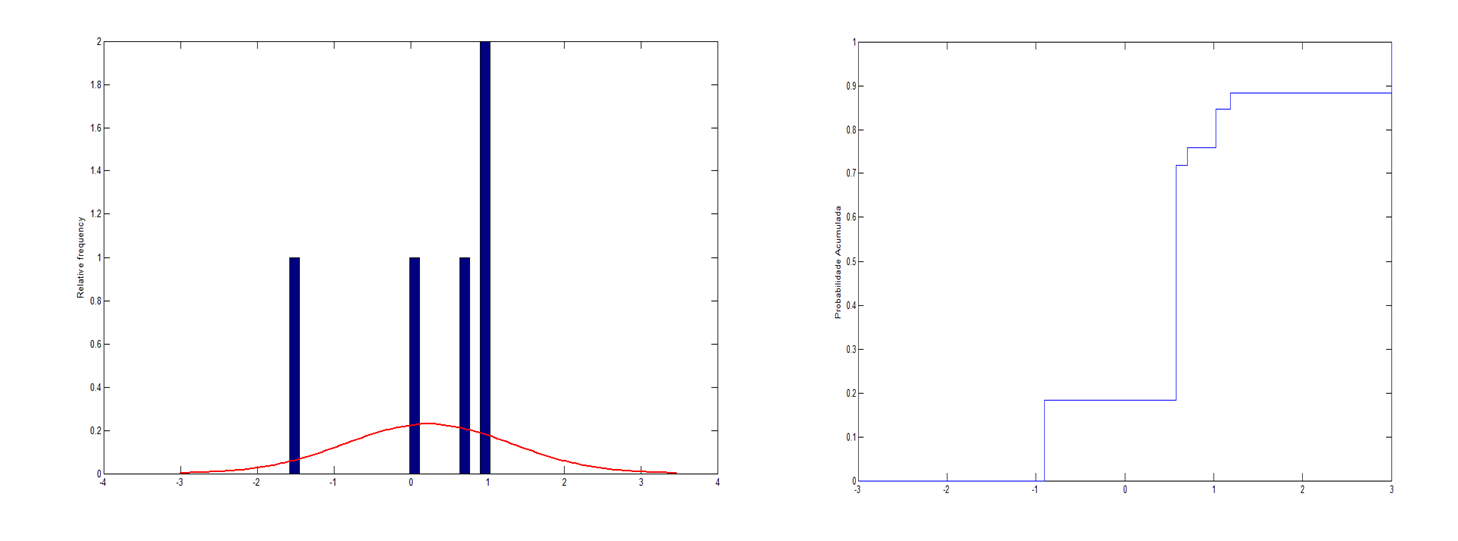
\includegraphics[scale=0.6]{aula10_10}\protect\caption{\label{fig:aula10_10} 5 cenários}
\end{centering}
\end{figure}
\begin{figure}[H]
\begin{centering}
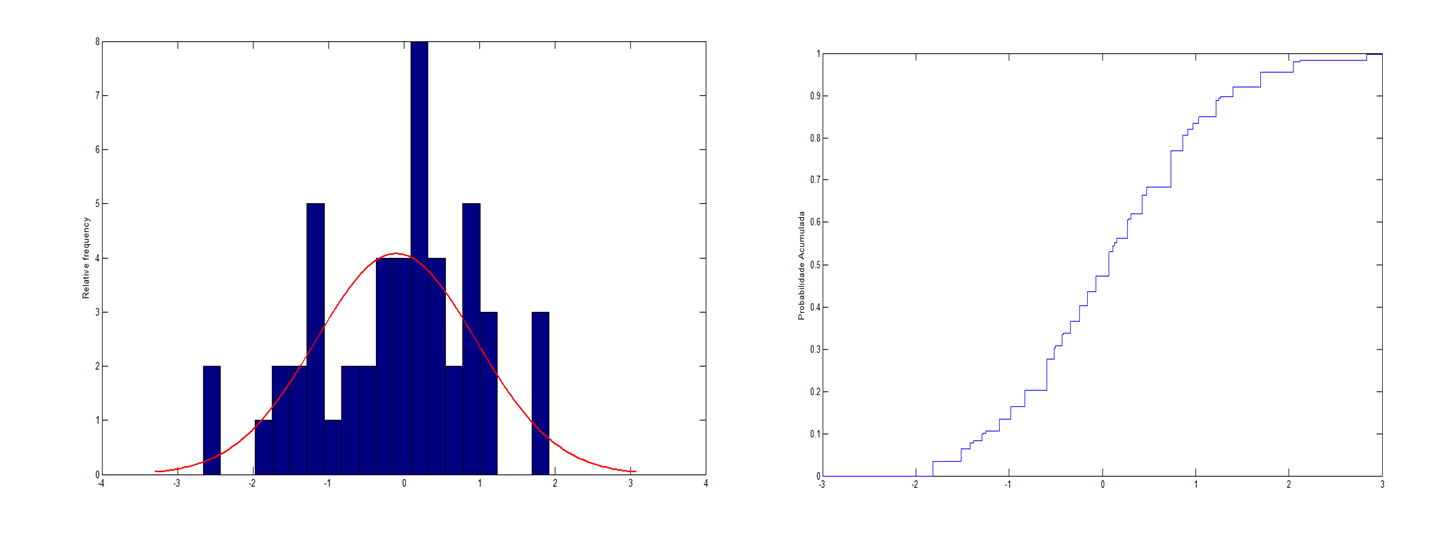
\includegraphics[scale=0.6]{aula10_11}\protect\caption{\label{fig:aula10_11} 50 cenários}
\end{centering}
\end{figure}
\begin{figure}[H]
\begin{centering}
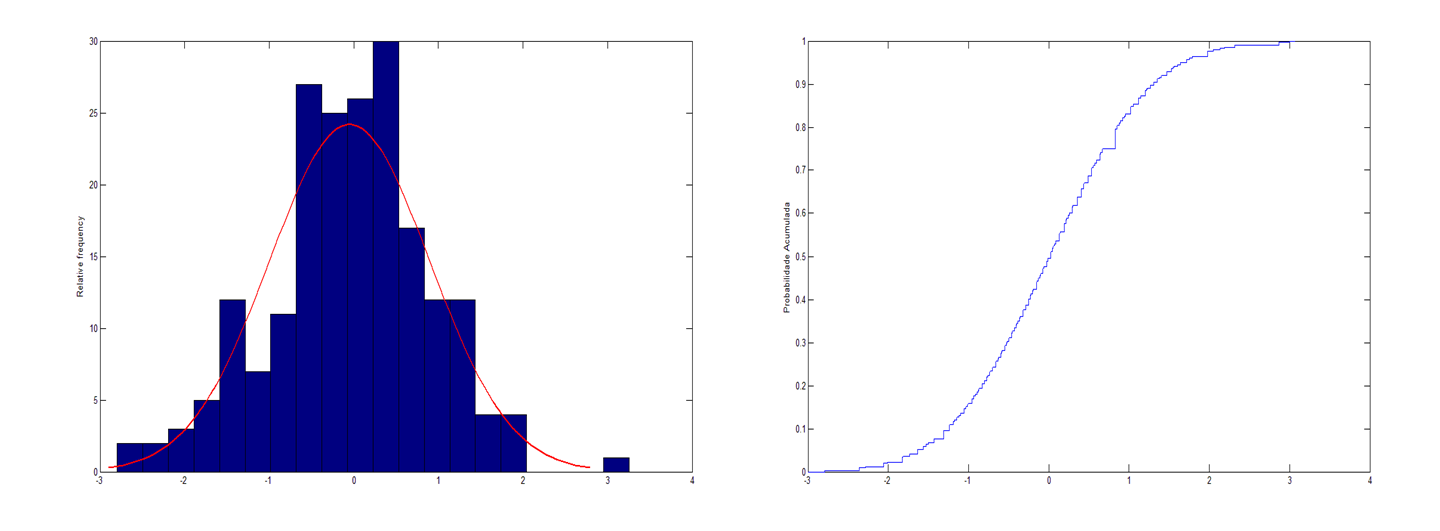
\includegraphics[scale=0.6]{aula10_12}\protect\caption{\label{fig:aula10_12} 200 cenários}
\end{centering}
\end{figure}
\begin{figure}[H]
\begin{centering}
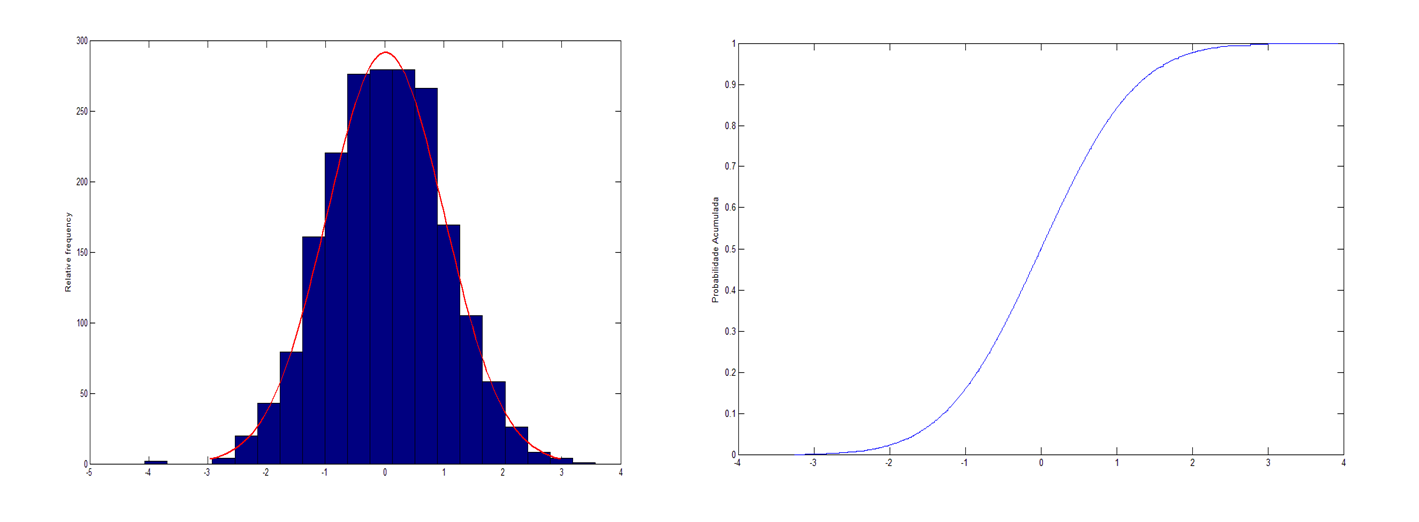
\includegraphics[scale=0.6]{aula10_13}\protect\caption{\label{fig:aula10_13} 2000 cenários}
\end{centering}
\end{figure}

 Assim, a convergência dos parâmetros,média e desvio padrão são representados pela figura\ref{fig:aula10_14}, onde apontamos a convergência em relação a quantidade de simulações. Aproximando para zero que é a média teórica e a variância tendendo para um que é a variância teórica. 
\begin{figure}[H]
\begin{centering}
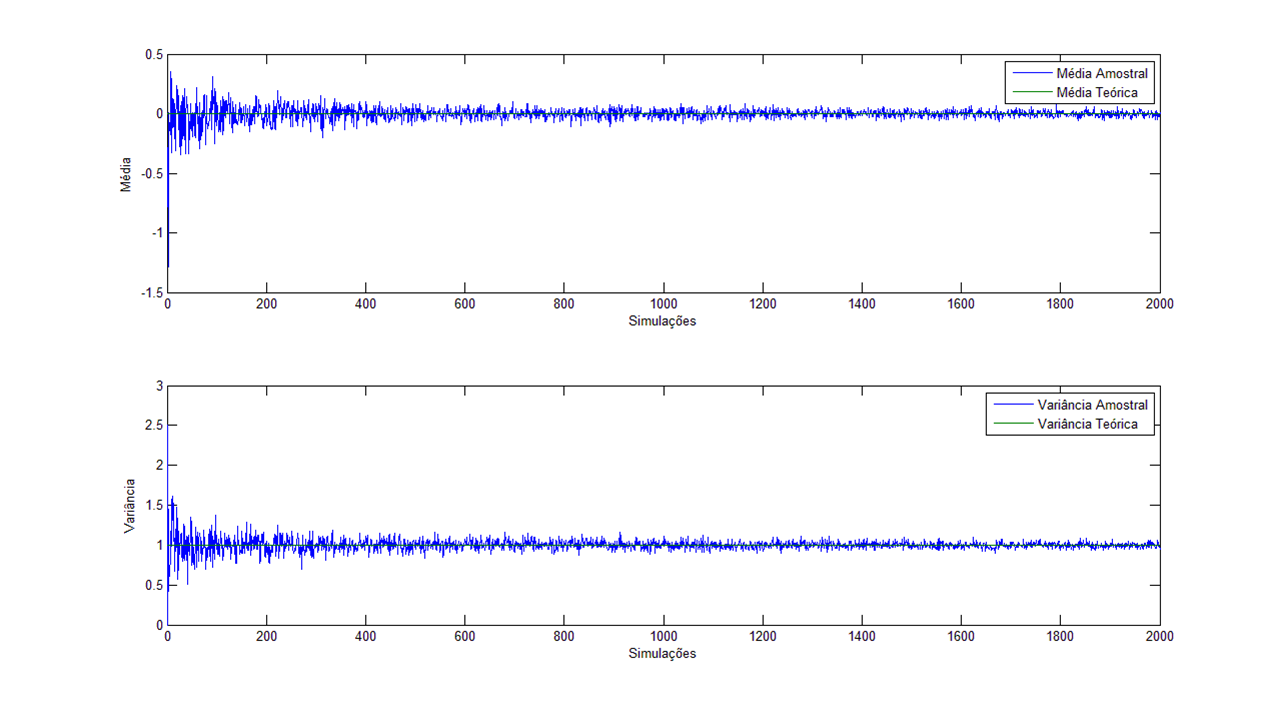
\includegraphics[scale=0.6]{aula10_14}\protect\caption{\label{fig:aula10_14} Convergência dos dados}
\end{centering}
\end{figure}

\subsection{Risco e Medida de risco}
 Risco é algo complicado para se definir mas de maneira geral podemos dizer que é a probabilidade e impacto de resultados desfavoráveis, o risco está atrelado à probabilidade de eventos desfavoráveis. Outro conceito que será utilizado é a incerteza onde é um conceito mais amplo que risco que envolve eventos para os quais não se sabe caracterizar a probabilidade de ocorrência.
 Nesta disciplina abordaremos o risco atrelado no ato da contratação que pode ser verificado no preço e quantidade, submercado, crédito e regulatório.
  
  O riscos de preço e quantidade é a incerteza no preço spot e na geração $R=P\cdot Q+(\tilde{g}-Q)\cdot\tilde{\pi}$, pode ser representado com a chance de não produzir o que foi prometido ,ou seja, a geração ser inferior ao montante contratado e preço spot alto. 
  Por exemplo, $Q=100MWh$, $g=50MWh$,$P=100\$/MWh$ e $\pi=250\$/MWh$.
  Temos,
$$ R=100\cdot 100+(50-100)\cdot 250=10.000-12.500=-2500,00 $$
Assim, temos uma renda negativa por ter produzido menos no contrato comprando o deficit de geração a um preço muito alto. O fator de risco nesse problema é o preço spot.

\begin{figure}[H]
\begin{centering}
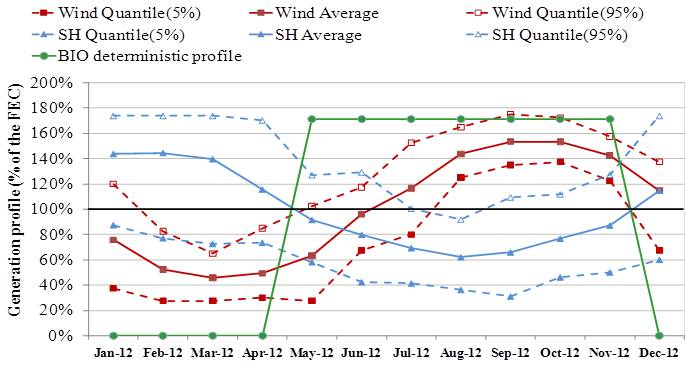
\includegraphics[scale=0.9]{aula10_15}\protect\caption{\label{fig:aula10_15}Perfil de Geração }
\end{centering}
\end{figure}

\begin{figure}[H]
\begin{centering}
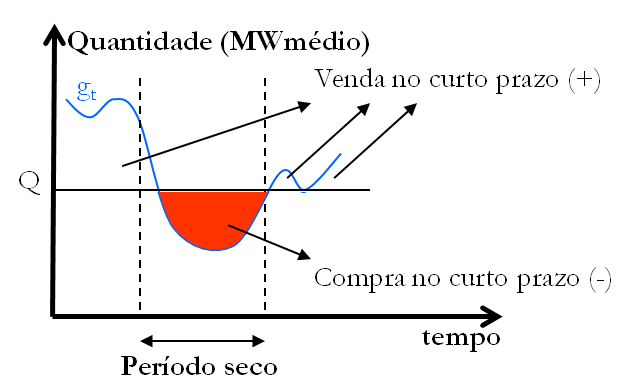
\includegraphics[scale=0.9]{aula10_16}\protect\caption{\label{fig:aula10_16} Quantidade de geração X Tempo}
\end{centering}
\end{figure}
 Para a ocorrência do risco de preço e quantidade é necessária a incertezas na produção, assim existem motivos que são mais comuns como as paradas forçadas ou programadas (por exemplo: máquina quebrada, manutenção com um preço de spot alto no mercado), a indisponibilidade de combustível ou insumo e energia renováveis que são o tempo todo expostas a esse risco por ter perfil sazonal a a disponibilidade depende de um fator exógeno,em especial as hidrelétricas em um sistema hidrotérmico onde, é negativamente correlacionada a geração hídrica e o preço spot .

\begin{figure}[H]
\begin{centering}
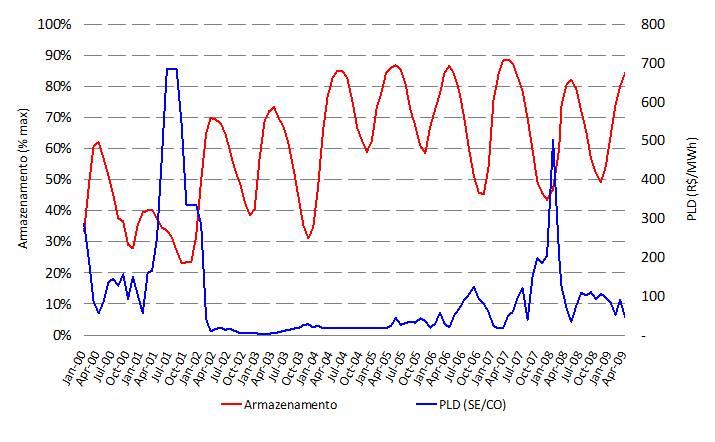
\includegraphics[scale=0.8]{aula10_17}\protect\caption{\label{fig:aula10_17} Armazenamento e PLD de Jan/00 até Abr/09 }
\end{centering}
\end{figure}
\begin{figure}[H]
\begin{centering}
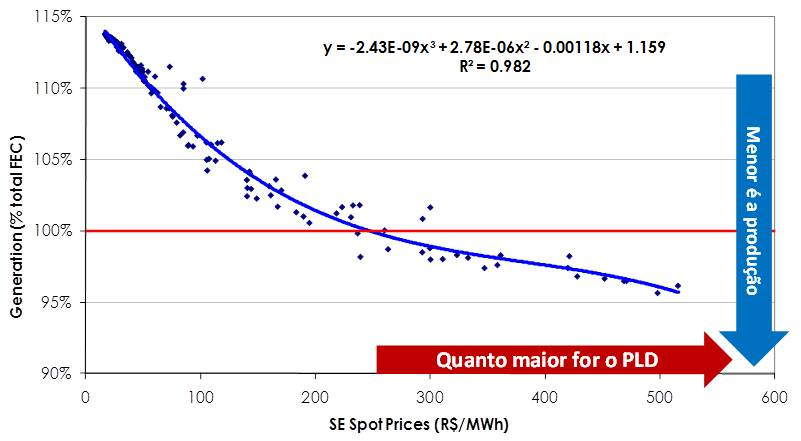
\includegraphics[scale=0.8]{aula10_18}\protect\caption{\label{fig:aula10_18} Geração X Preço de Spot}
\end{centering}
\end{figure}

 Para a caracterização do risco de preço e quantidade para as renováveis, é necessário uma simulação conjunta, de variáveis geração ($\tilde{g}$ ) e preço spot ($\tilde{\pi}$ ), figura \ref{fig:aula10_19}.


\begin{figure}[H]
\begin{centering}
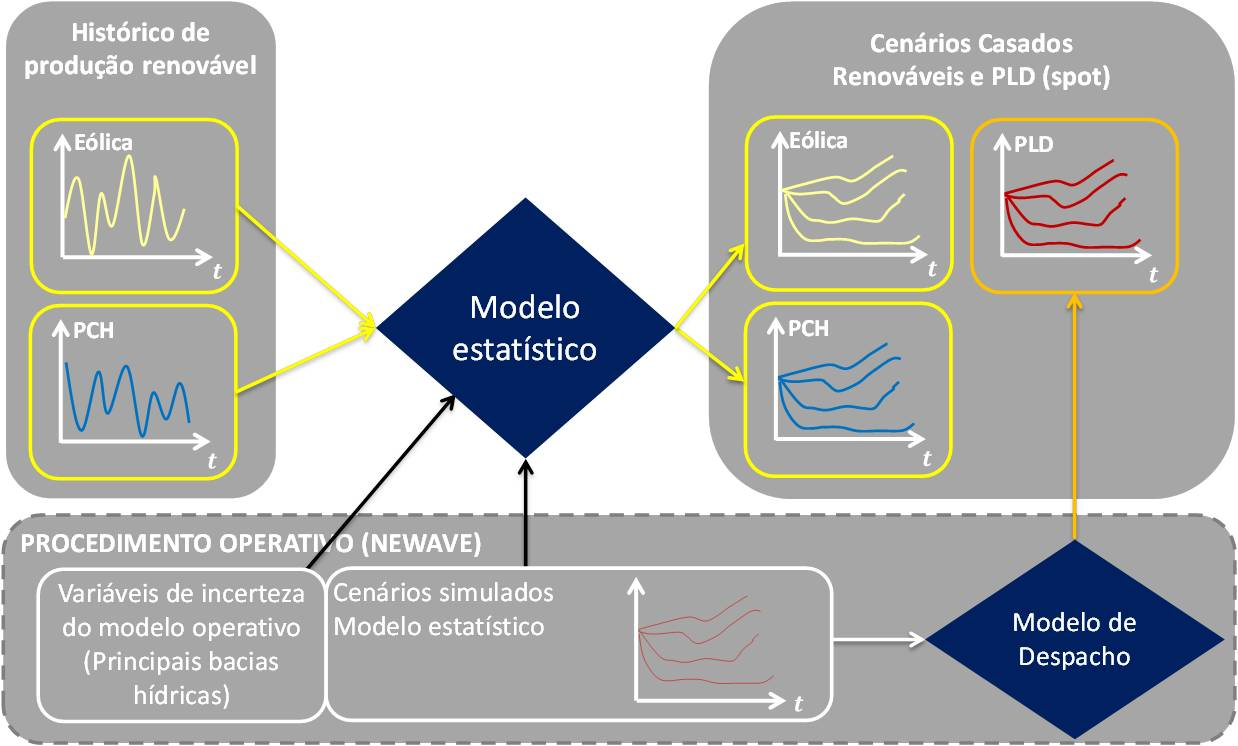
\includegraphics[scale=0.6]{aula10_19}\protect\caption{\label{fig:aula10_19} Modelo estatístico para caracterizar o risco }
\end{centering}
\end{figure}
  O risco de diferença de preço ocorre ao firmar um contrato com entrega numa barra diferente da barra de geração, é gerido quando a barra de geração tem um preço spot menor que a barra de entrega de contrato. Para verificar o riscos de diferença de preços entre submercados são representados no exemplo abaixo onde o contrato é feito com entrega na barra B e a geração é realizada na barra A,$\pi_{A}<\pi_{B}$ e a capacidade máxima de transmissão é esgotada na barra A para a barra B,figura \ref{fig:aula10_20}.
  Então, suponha um gerador 1 que venda um contrato para a 
 demanda 2,ou seja o produtor está na barra A e o consumidor na barra B. O gerador 1 vendeu um contrato com entrega no consumidor 2 e a expressão de renda será mais complexa, pelo fato da geração ser liquidada pela geração na barra A ($\pi_{A}$) e o contrato liquidado na barra B ($\pi_{B}$).
 Temos que,
 $R=P\cdot Q+(\tilde{g}\cdot\tilde{\pi_{A}}-Q\cdot\tilde{\pi_{B}}).$
 
 
\begin{figure}[H]
\begin{centering}
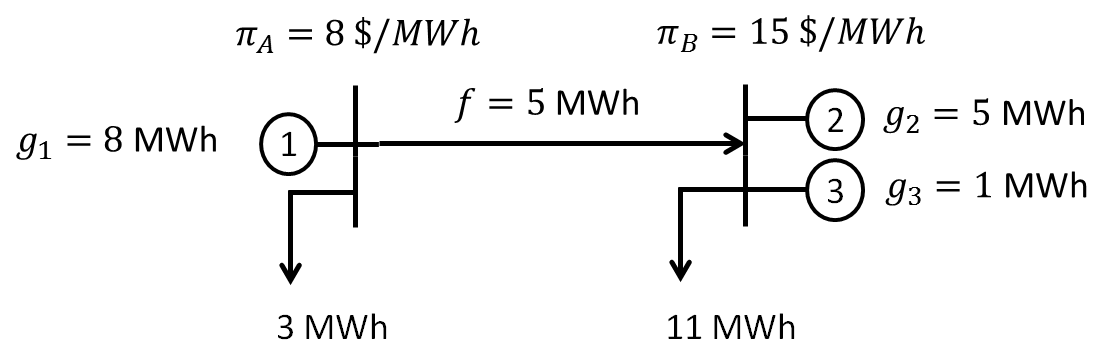
\includegraphics[scale=0.6]{aula10_20}\protect\caption{\label{fig:aula10_20} Exemplo risco de diferença}
\end{centering}
\end{figure}

\begin{figure}[H]
\begin{centering}
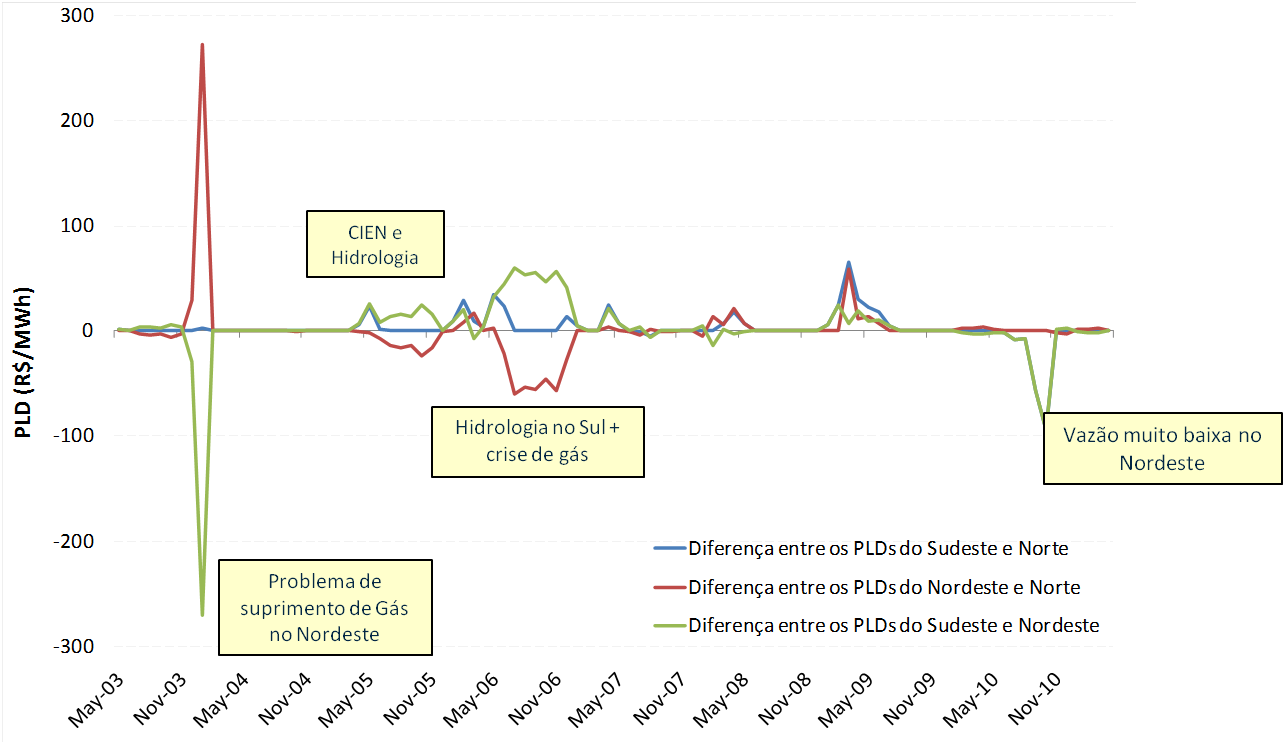
\includegraphics[scale=0.6]{aula10_21}\protect\caption{\label{fig:aula10_21} Diferença de preço spot entre o Norte, Nordeste e Sudeste}
\end{centering}
\end{figure}

O surplus de pagamento dos consumidores para os geradores é decorrente dos consumidores pagarem uma energia que foi liquidada para um valor mais baixo então a diferença de preço spot vezes o fluxo que passou na linha é o surplus de pagamento e é decorrente do limite de transmissão se não houvesse limite de transmissão toda energia ficaria igual do gerador mais caro. O limite da linha criou a diferença de preços, toda vez que houver uma linha garga lada criará a diferença de preço entre as barras que estão ligadas por essa linha então sempre que houver um gerador vendendo o contrato numa barra importadora ,por um preço de spot mais caro, esse gerador vai perder dinheiro no risco. 

\begin{figure}[H]
\begin{centering}
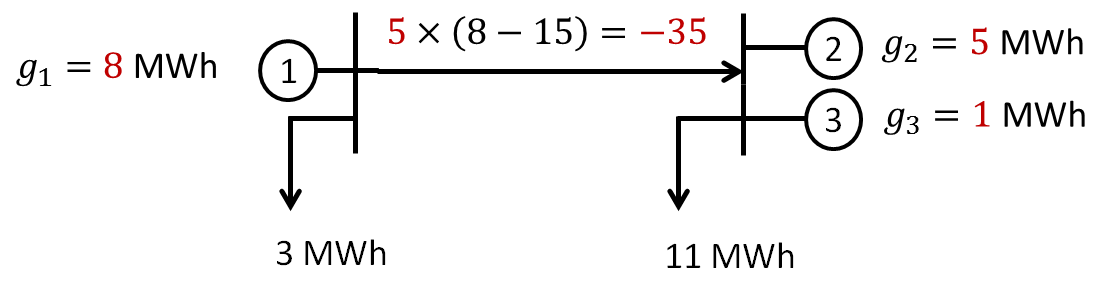
\includegraphics[scale=0.6]{aula10_22}\protect\caption{\label{fig:aula10_22} Despacho exemplo risco de diferença }
\end{centering}
\end{figure}

\begin{tabular}{|c|c|c|c|c|}
\hline 
 & Geração g MWh & Consumo D MWh & Spot $\pi$$\$/MWh$ & Receita/Despesa $g\times\pi$ou $-D\times\pi$ $\$$\tabularnewline
\hline 
\hline 
$G_{1}$ & 8 &  & 8 & $8\times8=64$\tabularnewline
\hline 
$G_{2}$ & 5 &  & 15 & $5\times15=75$\tabularnewline
\hline 
$G_{3}$ & 1 &  & 15 & $1\times15=75$\tabularnewline
\hline 
$D_{1}$ &  & 3 & 8 & $-3\times8=-24$\tabularnewline
\hline 
$D_{2}$ &  & 11 & 15 & $-11\times15=-165$\tabularnewline
\hline 
Fechamento & 14 & 14 &  & $soma=-35$\tabularnewline
\hline 

\end{tabular}

 O Hedge para o risco de submercado é se o gerador se contrata em outro subsistema tendo:

$R=P\cdot Q+(\tilde{g}\cdot\tilde{\pi_{A}}-Q\cdot\tilde{\pi_{B}}),$
decompondo os fatores de risco temos(preço e quantidade) e (diferença de preços - submercado), temos que,

$R=P\cdot Q+(\tilde{g}\cdot\tilde{\pi_{A}}-\tilde{g}\cdot\tilde{\pi_{B}}+\tilde{g}\cdot\tilde{\pi_{B}}-Q\cdot\tilde{\pi_{B}})$

$R=P\cdot Q+(\tilde{\pi_{A}}-\tilde{\pi_{B}})\cdot\tilde{g}+(\tilde{g}-Q)\cdot\tilde{\pi_{B}}.$

 O surplus de pagamento é um hedge perfeito para o risco de submercado é $S=-f\cdot(\tilde{\pi_{A}}-\tilde{\pi_{B}})$.
  Temos que, $S$ é um fato de risco em cada cenário, então o surplus de pagamento vai para os transmissores e esta transmissora vende um contrato para os geradores que querem se contratar com outros consumidores em outros subsistemas de maneira que este contrato pague o quanto o transmissor vai perder de dinheiro ou seja o inverso de $S$.

\begin{figure}[H]
\begin{centering}
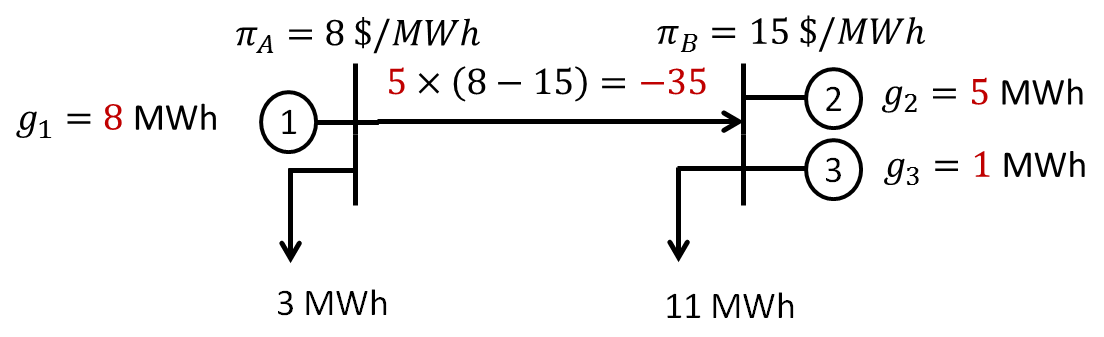
\includegraphics[scale=0.6]{aula10_23}\protect\caption{\label{fig:aula10_23} PLD por barra no exemplo risco de diferença }
\end{centering}
\end{figure}

 O riscos de crédito é o risco do comprador não pagar o contrato, onde esse "calote" é rateado entre os credores. Temos,

$$R=XPQ+(\tilde{g}-Q)\cdot\tilde{\pi}$$

$$X:\Omega\rightarrow[0,1],$$

e o risco de inadimplência no mercado,
$$
R=PQ+Y\cdot(\tilde{g}-Q)\cdot\tilde{\pi},
$$
onde, $Y:\varOmega\rightarrow[0,1]$ é o rateio das inadimplências entre os credores e $Y<$1 quando $\tilde{g}-Q>0$ com devedores inadimplentes.

\begin{figure}[H]
\begin{centering}
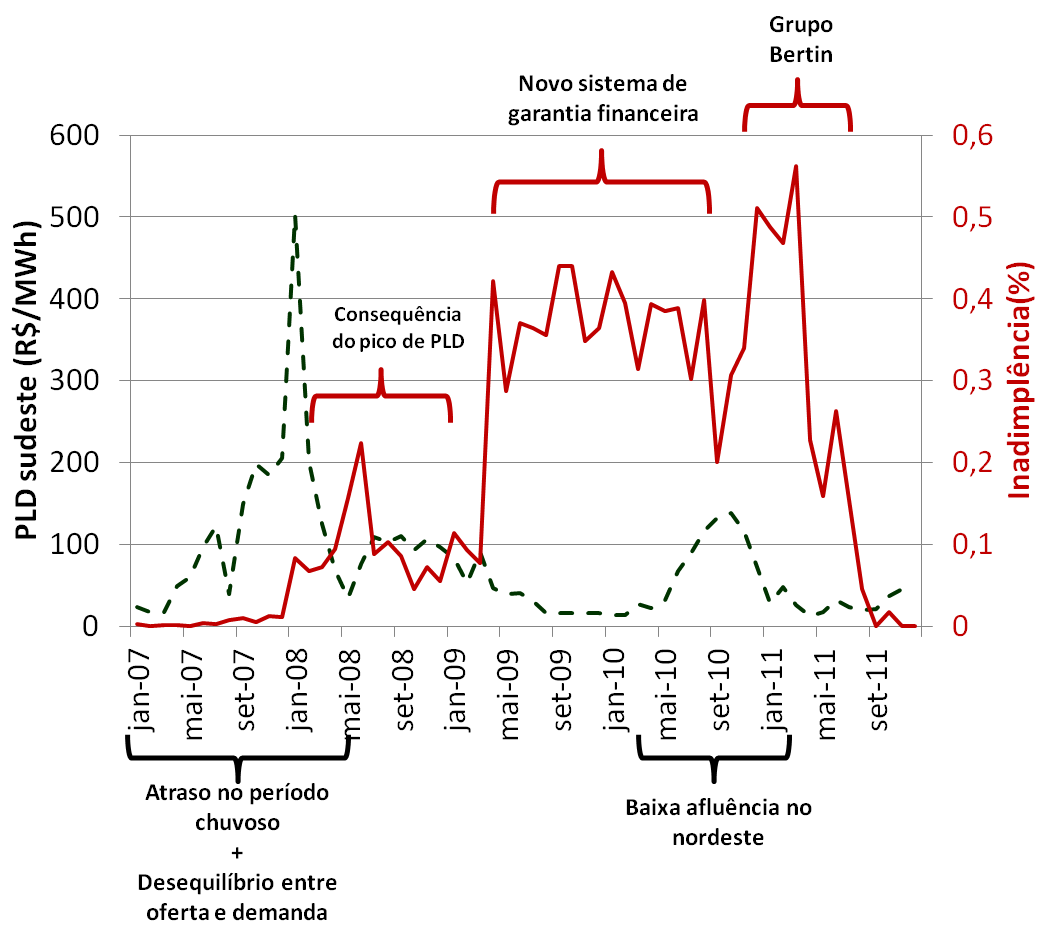
\includegraphics[scale=0.6]{aula10_24}\protect\caption{\label{fig:aula10_24} Risco de inadimplência no mercado}
\end{centering}
\end{figure}
  Em todo contrato existem dois lados, o lado de redução de risco e trás desafios a serem vencido, como a caracterização do risco trazendo uma estratégia de contratação ótima.
 Assim, os contratos são capazes de reduzir o risco e trazem desafios com relação as características dos riscos, necessária a estratégia de otimização e caracterização do perfil de risco. Para isso existe a gerência de risco na contratação, para que  existem propriedades desejáveis para o processo decisório corporativo. Com responsabilidade e aversão a risco definida em conselho,transparência no processo de decisão auditável e reprodutível e confiável que pode ser testado e simulado ex-ante, minimiza o fator emocional a hora da tomada de decisão.

 A aversão a risco pode ser representada pela figura \ref{fig:aula10_26}.

\begin{figure}[H]
\begin{centering}
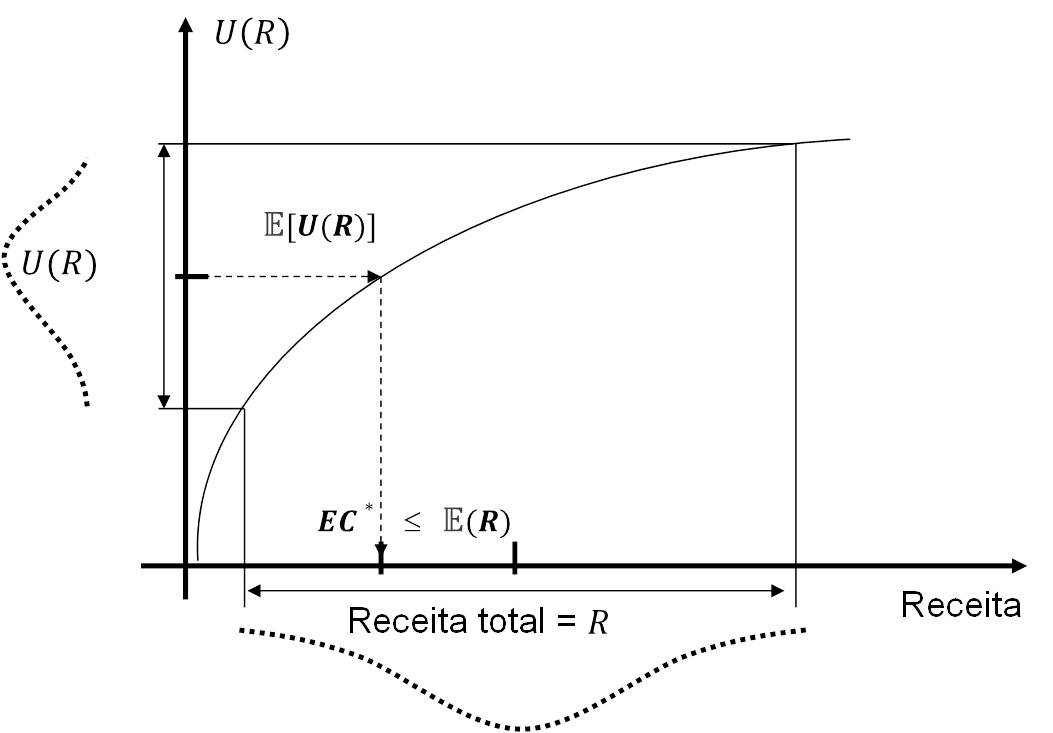
\includegraphics[scale=0.6]{aula10_26}\protect\caption{\label{fig:aula10_26} Primeira loteria}
\end{centering}
\end{figure}

\textbf{Exemplo}
 Para atribuir valor e será aplicado um exemplo, suponha que você ganhou uma entrada (ticket - direito) para um jogo em que uma moeda será lançada e caso a face coroa seja revelada, você ganha 1.000.000,00 R\$, caso contrário, você não ganha nada. Qual o menor valor monetário pelo qual você estaria disposto a vender a sua entrada?
\begin{figure}[H]
\begin{centering}
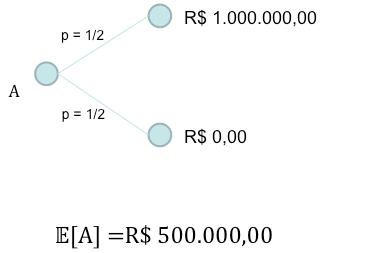
\includegraphics[scale=0.6]{aula10_27}\protect\caption{\label{fig:aula10_27} Segunda loteria}
\end{centering}
\end{figure}


E se você fosse convidado para este novo jogo? Qual seria o menor valor pelo qual você venderia a sua entrada?

\begin{figure}[H]
\begin{centering}
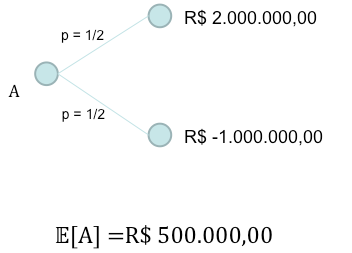
\includegraphics[scale=0.6]{aula10_28}\protect\caption{\label{fig:aula10_28} Terceira loteria}
\end{centering}
\end{figure}

Agora neste terceiro jogo seria, Quanto você pagaria para sair desse jogo?

\begin{figure}[H]
\begin{centering}
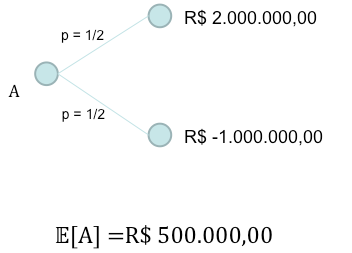
\includegraphics[scale=0.6]{aula10_29}\protect\caption{\label{fig:aula10_29} Escolha das loterias}
\end{centering}
\end{figure}


Então, em cada uma das loterias você deve escolher uma opção apresentadas na figura \ref{fig:aula10_31} com o respctivo perfil do agente.

\begin{figure}[H]
\begin{centering}
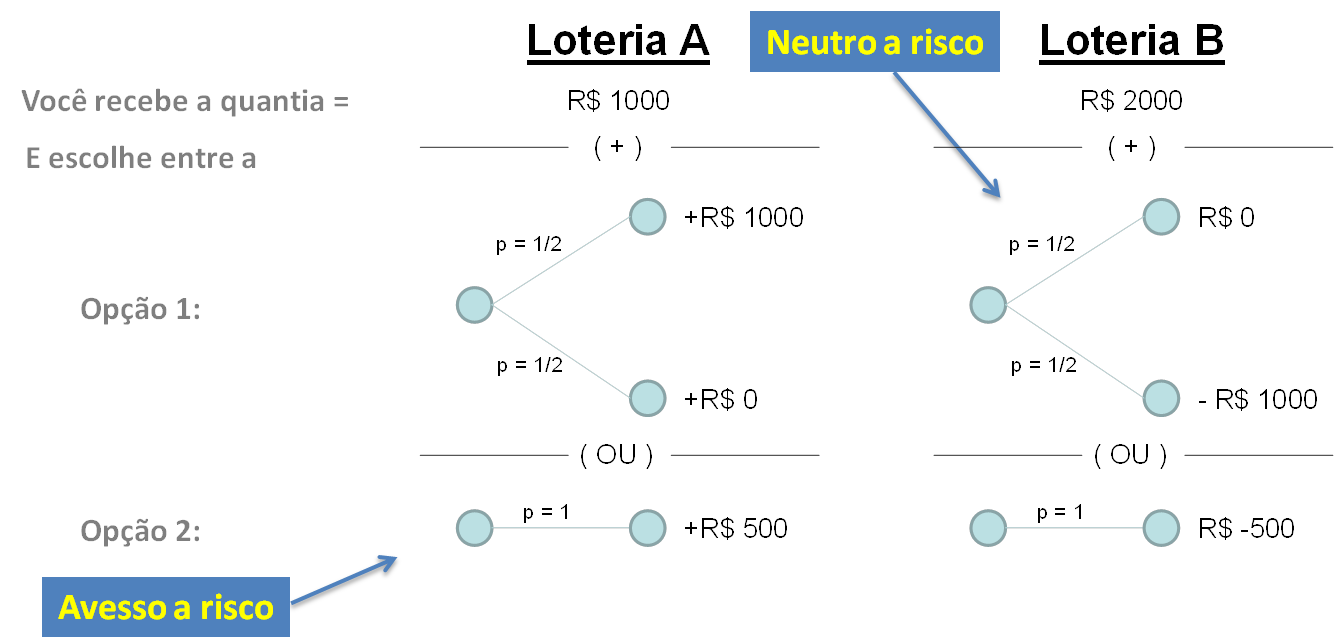
\includegraphics[scale=0.6]{aula10_31}\protect\caption{\label{fig:aula10_31} Escolha dependendo do perfil do agente}
\end{centering}
\end{figure}

Assim, como ambas as loterias possuem os mesmos cenários, deve selecionar opções diferentes representa um paradoxo no processo decisório.
 Como a abordagem de utilidade esperada se mostrou pouco prática para realizar decisões financeiras do dia-a-dia, a abordagem financeira, denominada Finanças, abriu portas para medir quantitativamente o risco de cada instrumento, sempre em unidades
monetárias. Assim finanças atrelado a otimização do problema é um poderoso instrumento para a tomada de decisão empresarial.
 
 Retomando a parte conceitual de teoria da decisão e risco, o valor ou equivalente certo, atribui um valor monetário (em uma determinada data, por exemplo, hoje) pelo qual estaríamos indiferentes entre este montante e tal oportunidade. Vamos utilizar medidas de risco ou utilidades para encontrar o valor,ou equivalente certo, de um determinado projeto.E o fluxo de caixa são conjuntos de variáveis aleatórias parametrizadas em decisões.

 A medida de risco tem como objetivo reduzir o risco, em geral, que afeta o retorno esperado. Nos protegendo de eventos adversos, normalmente, reduzindo o retorno esperado da comercialização (Trade-off entre Risco e Retorno Esperado \textendash{}Markovitz). Assim, buscamos indicadores que quantifiquem o risco pra otimizar
as decisões considerando este trade-off entre risco e retorno esperado. Existem diversos indicadores propostos para medir o risco, a variância e o desvio padrão, valor em risco (VaR) e valor em risco condicional (CVaR).
\subsubsection{Desvio Padrão}
 Utilizar o desvio padrão como medida de risco tem como objetivo do tomador de decisão dados que estejam com pequenas dispersão em torno da média entre as loterias propostas. Assim o desvio padrão é dado por:

\[
\sigma=\sqrt{\int(X(\omega)-\mu)^{2}dF_{x}(\omega)}.
\]
\begin{figure}[H]
\begin{centering}
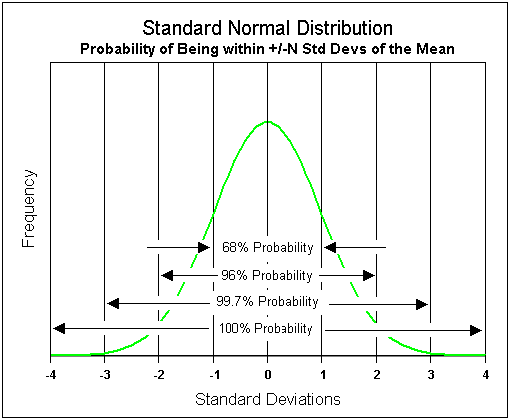
\includegraphics[scale=0.6]{aula10_32}\protect\caption{\label{fig:aula10_32} Desvio padrão}
\end{centering}
\end{figure}

\subsubsection{Value at Risk} 
 O Value at Risk - VaR é o quantil pessimista da distribuição de renda, o montante em caixa necessário para cobrir$\alpha$ dos casos.Seja $(\varOmega,\mathcal{F},\mathbb{P})$ um espaço de probabilidades
e $X\in\chi$ uma variável aleatória que representa o fluxo financeiro
de um investimento A métrica Value-at-Risk é um funcional $VaR_{\alpha}:\chi\rightarrow\mathbb{R}$
definido como: 
\[
VaR_{\alpha}(X)=min\{z\in\mathbb{R}|\mathbb{P}(\{\omega\in\varOmega|X(\omega)+z\leq1-\alpha,
\]
onde $\alpha\in(0,1)$ é conhecido como nível de significância. Valores
típicos para$\alpha$são 0.90, 0.95 e 0.99.

Assim, equivalentemente, observamos que o $VaR_{\alpha}$ está associado
ao ponto limite em que a área sob a curva de distribuição de probabilidade(figura \ref{fig:aula10_32})
é inferior ao Nível de Significância $1-\alpha.$ Intuitivamente,
ao adicionarmos um valor fixo a um fluxo financeiro, estamos \textquotedblleft empurrado\textquotedblright{}
sua curva de distribuição de probabilidade para a direita. Assim,
o $VaR_{\alpha}$ indica o montante financeiro faltante para que divida
a distribuição entre $1-\alpha$ e$\alpha$. Importante ressaltar
que esta métrica de risco depende apenas de uma especificação precisa
da cauda inferior da distribuição de probabilidade e está diretamente
ligada aos estados da natureza de pior performance do investimento,
estando, portanto, coerente com a intuição por trás do conceito de
risco.
\begin{figure}[H]
\begin{centering}
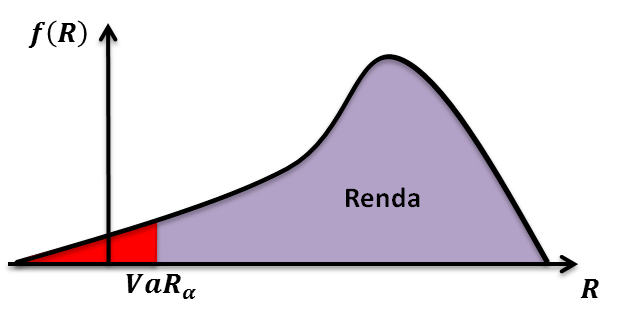
\includegraphics[scale=0.6]{aula10_33}\protect\caption{\label{fig:aula10_32} VaR}
\end{centering}
\end{figure}

\subsubsection{Conditional Value at Risk} 

    O conditional value at risk  (CVaR) é uma medida de risco que surgiu como uma alternativa mais interessante ao VaR. Um dos motivos é a dificuldade de modelar o VaR em um modelo de otimização,sendo necessária a utilização de variáveis inteiras gerando um problema não
convexo muito mais difícil de se resolver. Outros motivos, é que o VaR não captura a informação sobre a  cauda inferior da distribuição, não mede o risco (impacto) dos cenários catastróficos. Além disso, o CVaR é uma medida coerente de risco:$CVaR(A+B)\geq CVaR(A)+CVaR(B)$ e é simplesmente, a média condicional da renda abaixo do VaR, assim captura a existência de eventos pouco prováveis,porém devastadores.Pode ser facilmente incorporado em problemas de otimização pelo fato de ser convexo.
A figura \ref{fig:aula10_34} representa a distribuições com mesmo $VaR_{\alpha}$, com caudas
inferiores diferentes e a comparação do $CVaR_{\alpha}$, mostrando sua captura a presença de eventos abaixo do VaR e diferencia as duas distribuições.

\begin{figure}[H]
\begin{centering}
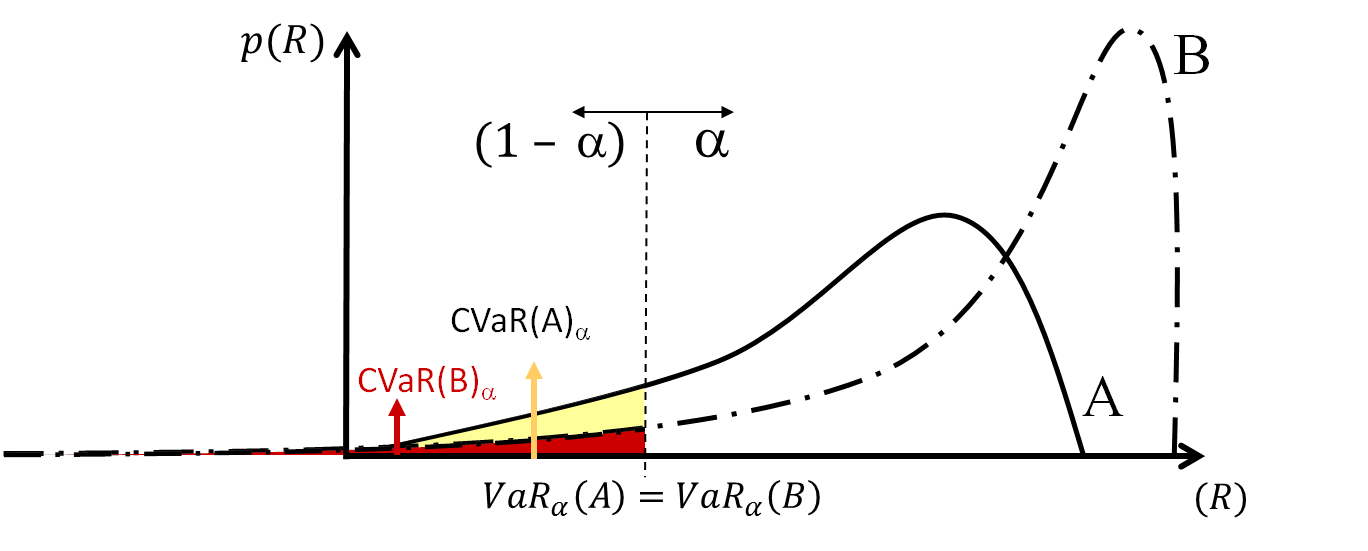
\includegraphics[scale=0.6]{aula10_34}\protect\caption{\label{fig:aula10_34} CVaR e VaR}
\end{centering}
\end{figure}

Podemos representar o CVaR como um modelo de otimização para a contratação da seguinte maneira,

\[
CVaR_{\alpha}(\tilde{R})=max_{z,\delta(\omega)\geq o}\left\{ z-\sum_{\omega\in\varOmega}p(\omega)\left(\frac{\delta(\omega)}{(1-\alpha}\right)|\delta(\omega)\geq z-R(\omega),\forall\omega\in\varOmega\right\} .
\]
\begin{figure}[H]
\begin{centering}
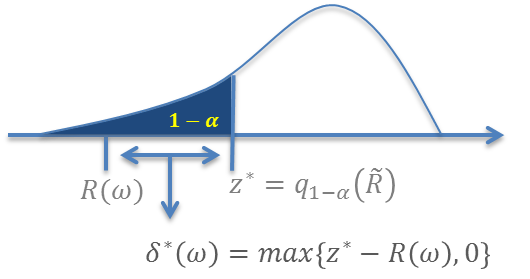
\includegraphics[scale=0.6]{aula10_35}\protect\caption{\label{fig:aula10_35} CVaR e média referente ao risco}
\end{centering}
\end{figure}

Uma medida de risco baseada no CVaR é a diferença entre a potencial perda e o que se espera,
$Risco(\tilde{R})=\mathbb{E}(\tilde{R})-CVaR_{\alpha}(\tilde{R})$, onde $\alpha$ é um parâmetro de aversão a risco.

\textbf{Exemplo}
Um exemplo é a contratação hidrelétrica, onde cada contrato de venda da geração hidrelétrica gera uma receita,$\tilde{R}(Q=1MWh,...,\tilde{R}(Q=10MWh)$,um preço de contrato = Média do spot $=240\ensuremath{/MWh}$ e uma receita média $=1360\ensuremath{\$}$.
\begin{figure}[H]
\begin{centering}
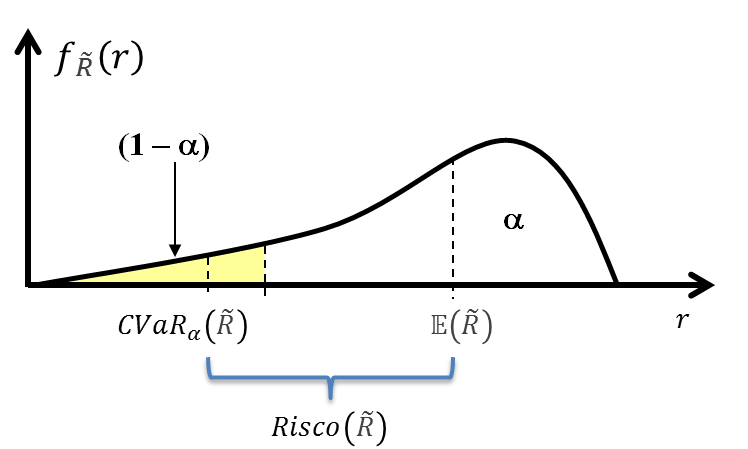
\includegraphics[scale=0.6]{aula10_36}\protect\caption{\label{fig:aula10_36} Exemplo de quantidade de contratos ótima}
\end{centering}
\end{figure}
\begin{figure}[H]
\begin{centering}
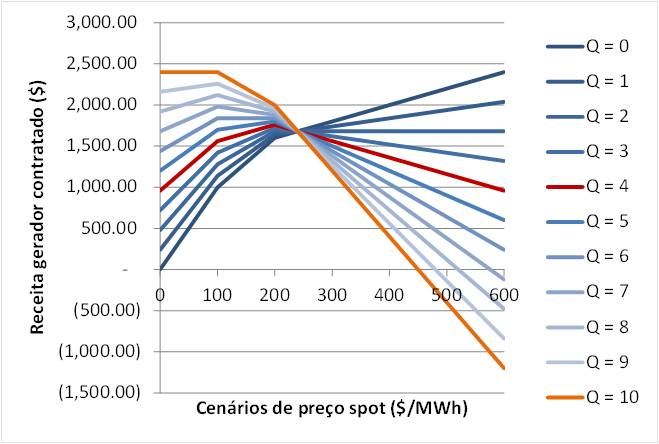
\includegraphics[scale=0.6]{aula10_37}\protect\caption{\label{fig:aula10_37} Exemplo de quantidade de contratos ótima com as medidas de risco}
\end{centering}
\end{figure}

\begin{figure}[H]
\begin{centering}
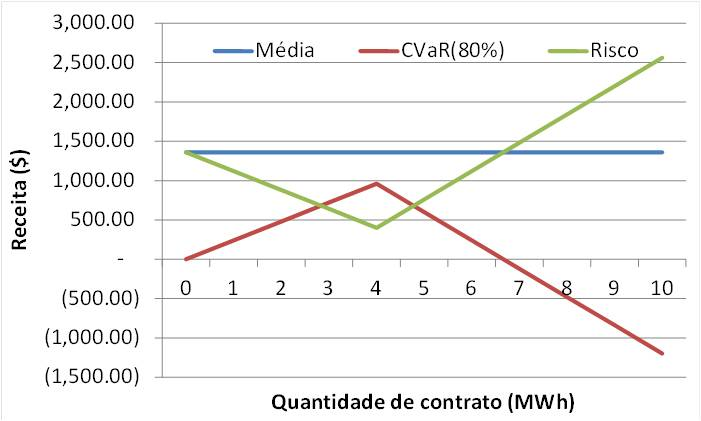
\includegraphics[scale=0.6]{aula10_38}\protect\caption{\label{fig:aula10_38} Gráfico quantidade de contrato x Receita}
\end{centering}
\end{figure}

 Ainda pode-se associar ao valor esperado ajustado ou penalizado pelo risco:

$$\mu(\tilde{R})=\lambda CVaR_{\alpha}(\tilde{R})+(1-\lambda)\mathbb{E}(\tilde{R}),$$

Onde, $\lambda\in[0,1]$ é um segundo parâmetro de aversão a risco.

Como propriedade da medida de valor baseada no CVaR é verificada a combinação convexa entre o CVaR (avessa a risco) e valor Esperado
(Neutra a risco) é,
\[
\mu(\tilde{R})=\lambda CVaR_{\alpha}(\tilde{R})+(1-\lambda)\mathbb{E}(\tilde{R}),
\]


\[
\mu(\tilde{R})=\mathbb{E}(\tilde{R})-\lambda[\mathbb{E}(\tilde{R})-CVaR_{\alpha}(\tilde{R})],
\]


\[
\mu(\tilde{R})=\mathbb{E}(\tilde{R})-\lambda Risco(\tilde{R}).
\]


E o decréscimo marginal de \textquotedblleft valor\textquotedblright{}
com um incremento marginal de risco

\[
\frac{\partial\mu(\tilde{R})}{\partial Risco(\tilde{R})}=\lambda.
\]

 Abaixo serão representados alguns conceitos de decisão de um determinado conjunto de portfólio através do gráfico gráfico de risco e retorno com o CVaR (figura \ref{fig:aula10_40}), onde, o eixo
 $y :\mathbb{E}(\tilde{R}(Q_{i}))$ e o eixo $x, Risco(\tilde{R}(Q_{i}))=\mathbb{E}(\tilde{R(Q_{i})})-CVaR_{\alpha}(\tilde{R(Q_{i})})$.
 
\begin{figure}[H]
\begin{centering}
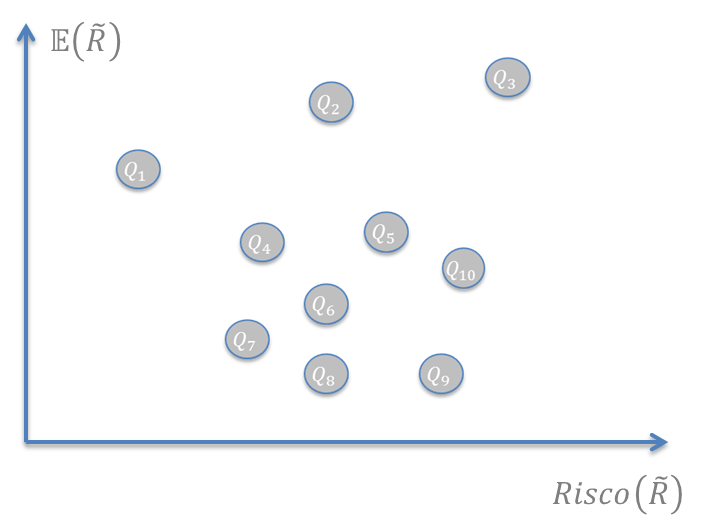
\includegraphics[scale=0.6]{aula10_40}\protect\caption{\label{fig:aula10_40} Gráfico risco e retorno com CVaR}
\end{centering}
\end{figure}


As decisões dominadas por $R(Q_{1})$ são para todo $i$ tal que, $\mathbb{E}(\tilde{R(Q_{i})})<\mathbb{E}(\tilde{R(Q_{1})})$ e $Risco(\tilde{R}(Q_{i}))>Risco(\tilde{R}(Q_{1}))$.

\begin{figure}[H]
\begin{centering}
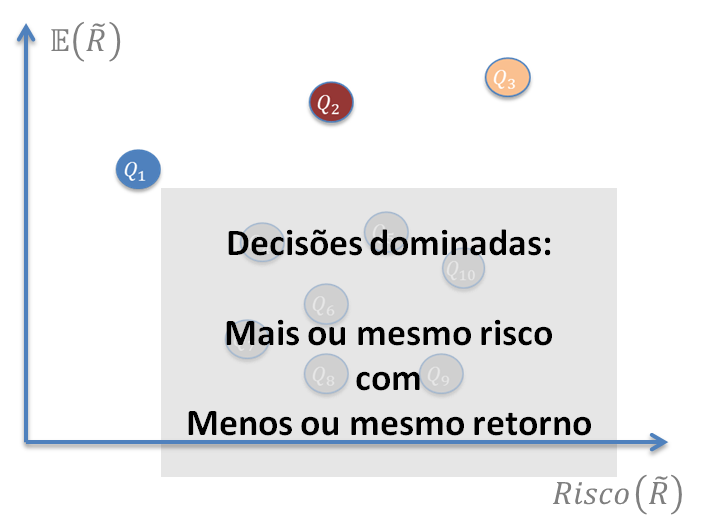
\includegraphics[scale=0.6]{aula10_41}\protect\caption{\label{fig:aula10_41} decisões dominadas}
\end{centering}
\end{figure}


A curva isovalor no plano Risco e Retorno é tal que para todo $\tilde{R}$ tal que $\mu(\tilde{R})=\mathbb{E}(\tilde{R})-\lambda Risco(\tilde{R})=\mu_{0}$
é igualmente preferível a $\tilde{R}(Q_{1})$,$\mathbb{E}(\tilde{R})=\mu_{0}+\lambda Risco(\tilde{R})$.

\begin{figure}[H]
\begin{centering}
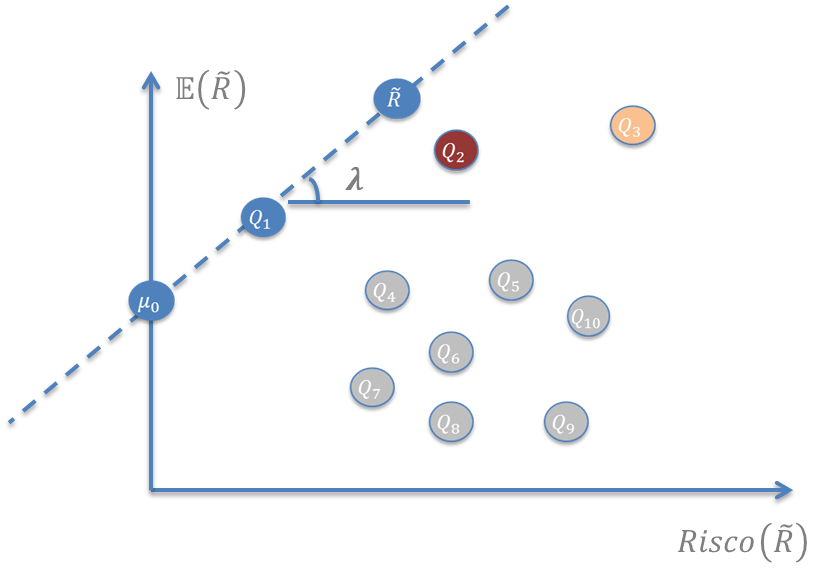
\includegraphics[scale=0.6]{aula10_42}\protect\caption{\label{fig:aula10_42} Curva isovalor}
\end{centering}
\end{figure}


 A fronteira eficiente é a solução de maior valor depende de $\lambda$, onde a preferência depende da aversão a risco e quanto aceitamos a mais de risco para um mesmo valor esperado (\ref{fig:aula10_41}) ou é o conjunto de pontos não dominados por nenhum outro ponto  (figura\ref{fig:aula10_42}), também podemos considerar como o conjunto de pontos para o qual existe um $\lambda$ para cada elemento que o torne o mais preferível e o conjunto de pontos de máximo valor esperado para cada nível de risco figura \ref{fig:aula10_43}.

Ou seja, a fronteira eficiente é dada por: 

$$max_{Q\in\mathbb{Q}}\lambda_{i}CVaR_{\alpha}\left(\tilde{R}(Q)\right)+(1-\lambda_{i})\mathbb{E}\left(\tilde{R(Q})\right).$$

\begin{figure}[H]
\begin{centering}
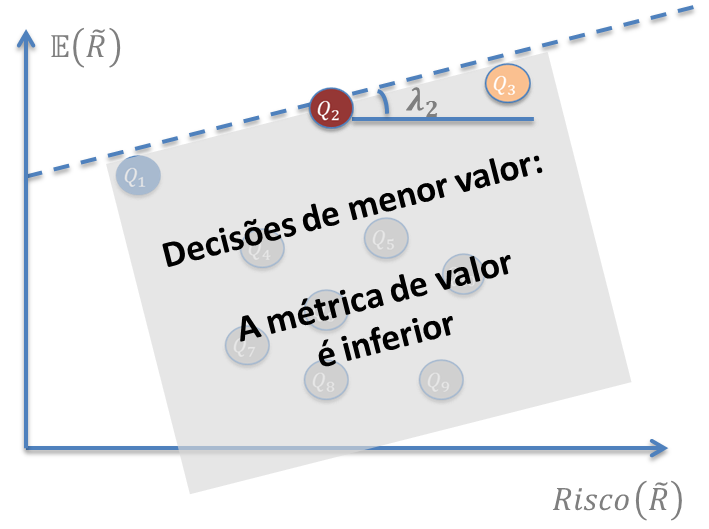
\includegraphics[scale=0.6]{aula10_43}\protect\caption{\label{fig:aula10_43} Decisão de menor valor }
\end{centering}
\end{figure}

Assim, o problema escrito como um problema de programação linear é,
$$max_{Q\in\mathbb{Q}}\mathbb{E}\left(\tilde{R(Q})\right)$$

$$s.a \quad Risco\left(\tilde{R}(Q)\right)\leq r.$$

\begin{figure}[H]
\begin{centering}
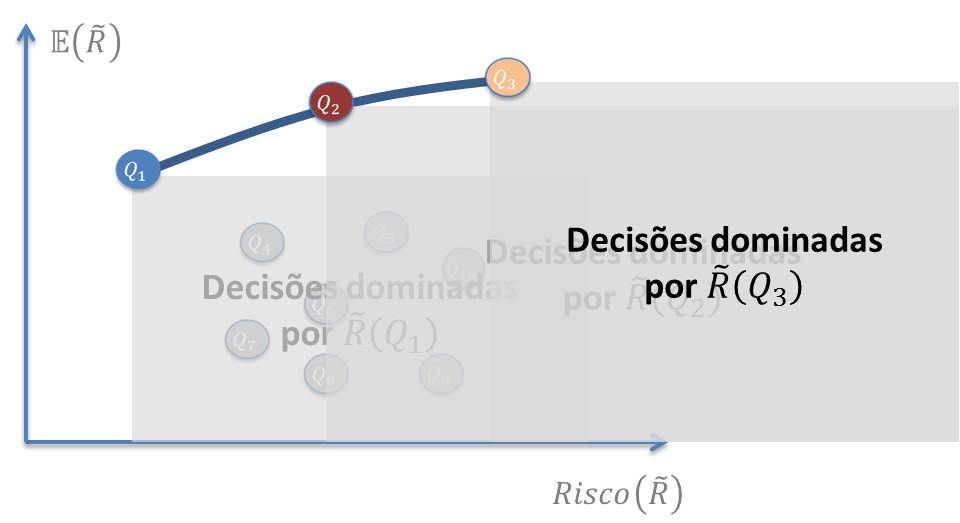
\includegraphics[scale=0.6]{aula10_44}\protect\caption{\label{fig:aula10_44} Decisão dominadas pelo contrato 3}
\end{centering}
\end{figure}

\begin{figure}[H]
\begin{centering}
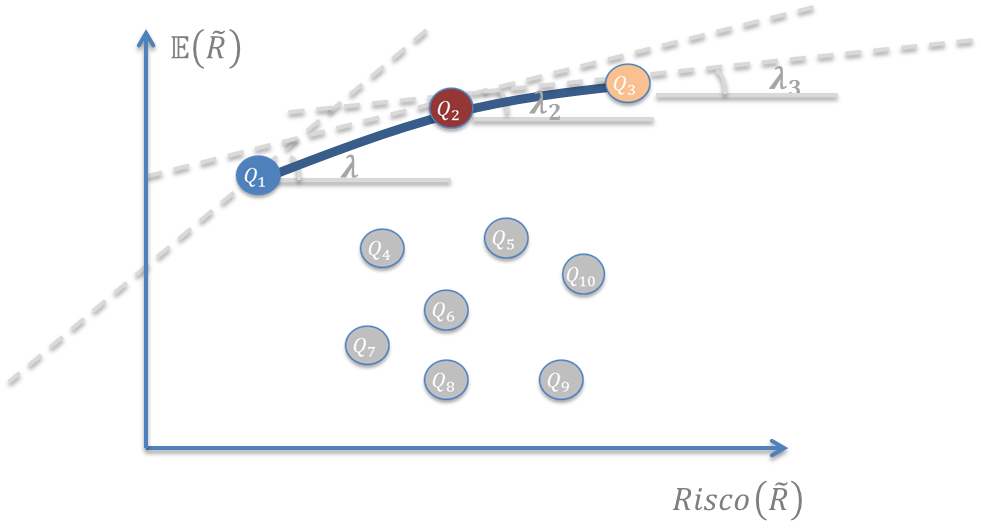
\includegraphics[scale=0.6]{aula10_45}\protect\caption{\label{fig:aula10_45} Gráfico de um $\lambda$ que torne o elemeto mais preferível}
\end{centering}
\end{figure}

\begin{figure}[H]
\begin{centering}
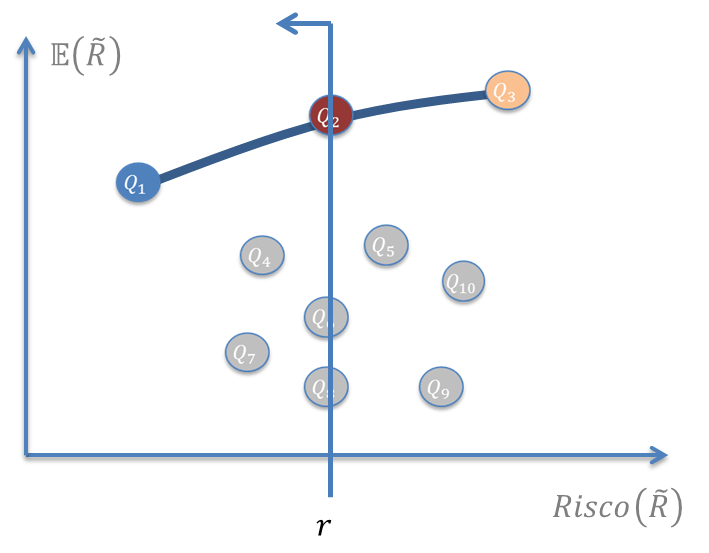
\includegraphics[scale=0.6]{aula10_46}\protect\caption{\label{fig:aula10_46} Ponto máximo para cada nível de risco}
\end{centering}
\end{figure}
\subsection{Otimização de contratos}
 A otimização de contratos pode ser representada pela figura (\ref{fig:aula10_47}) e é um problema de criação de um portfólio sob incerteza que seleciona dentro de um conjunto de oportunidades (contratos candidatos), um subconjunto que maximizar o valor, $\mu$, da renda
líquida final, $\tilde{R}(x)$, que é composta pela, renda líquida com contratos candidatos , $\tilde{R}^{C}(x)$,função das quantidades de contratos candidatos de venda e/ou compra , acrescida da receita dos contratos do portfolio existente, $\tilde{R}^{E}$, acrescidas das penalidades de sub contratação $\varPhi(x)$,onde $x=\left[Q_{1},...,Q_{n}\right]^{T}$é o vetor de quantidades dos contratos candidatos.
Temos que,
\[
\max_{x\in\mathbb{X}}\mu\left\{ \tilde{R}^{C}(x)+\tilde{R}^{E}+\varPhi(x)\right\} ,
\]


e pode ou não considerar restrições de risco,

\[
Risco\left\{ \tilde{R}^{C}(x)+\tilde{R}^{E}+\varPhi(x)\right\} \leq v .
\]

\begin{figure}[H]
\begin{centering}
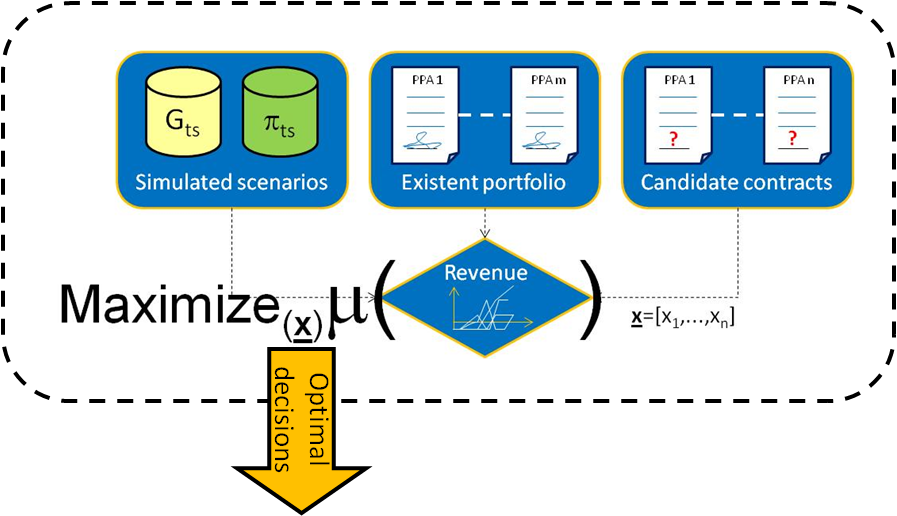
\includegraphics[scale=0.6]{aula10_47}\protect\caption{\label{fig:aula10_47}Otimização de contratos}
\end{centering}
\end{figure}

\textbf{Exemplo}
Suponha uma empresa com um gerador termelétrico com custo variável unitário igual a $150\ensuremath{\$/MWh}$
\[
\tilde{R}^{E}=\tilde{g}^{T}\tilde{\pi}.
\]
E que a empresa tenha duas oportunidades no mercado, a primeira de adquirir uma fração $x$ de uma hidrelétrica ao custo de $C=100\$/cota$ e a outra de vender um contrato de $Q$ $MWh$ para um consumidor livre pelo preço $P=200\$/MWh$, assim
\[
\tilde{R}^{C}(Q,x)=(P-\tilde{\pi})\cdot Q+(\tilde{g}^{H}\tilde{\pi}-C)\cdot x.
\]


\begin{tabular}{|c|c|c|c|c|c|}
\hline 
t & 1 & 2 & 3 & 4 & 5\tabularnewline
\hline 
\hline 
$\pi$ & 0 & 100 & 200 & 300 & 600\tabularnewline
\hline 
$\tilde{g}^{T}$ & 0 & 10 & 10 & 10 & 10\tabularnewline
\hline 
$\tilde{g}^{H}$ & 12 & 10 & 8 & 6 & 4\tabularnewline
\hline 
Prob & 0.2 & 0.2 & 0.2 & 0.2 & 0.2\tabularnewline
\hline 
\end{tabular}

Se por exemplos  compramos todas as cotas da hidro: $x=1$,

\[
\tilde{R}(Q,1)=(P-\tilde{\pi})\cdot Q+(\tilde{g}^{H}\tilde{\pi}-C)\cdot x+\tilde{g}^{T}\tilde{\pi},
\]


\[
\tilde{R}(Q,1)=PQ+(\tilde{g}^{H}+\tilde{g}^{T}-Q)\cdot\tilde{\pi}-C.
\]

\begin{figure}[H]
\begin{centering}
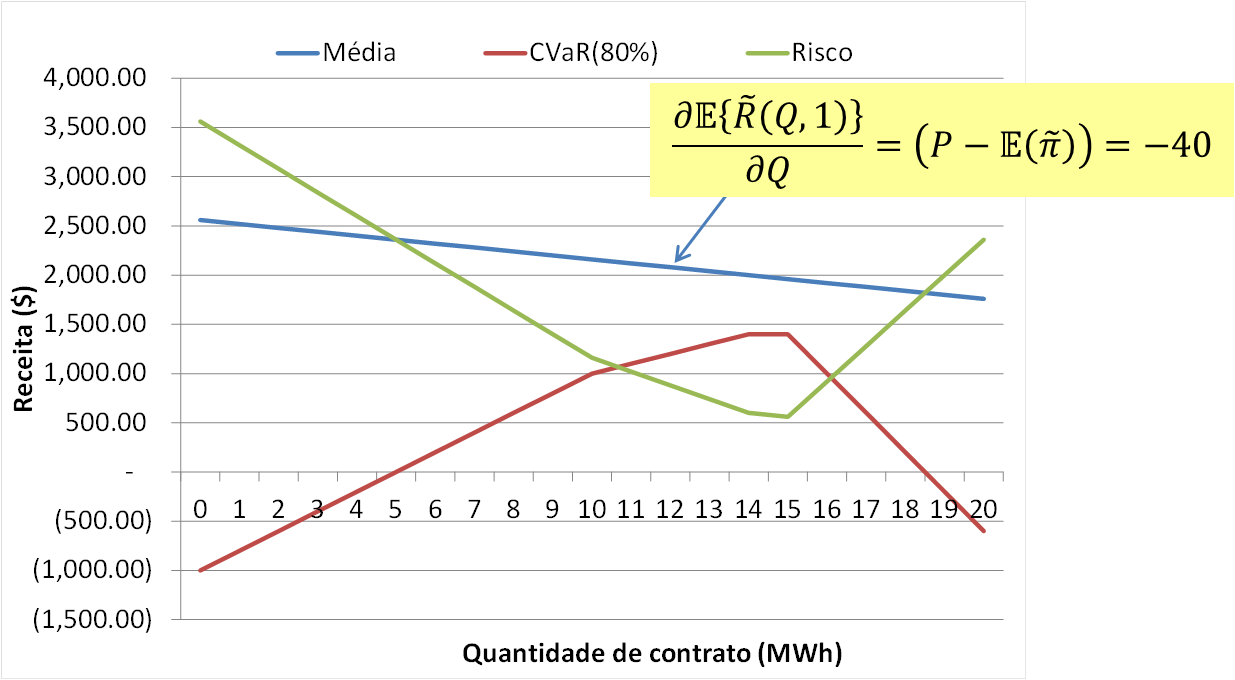
\includegraphics[scale=0.6]{aula10_48}\protect\caption{\label{fig:aula10_48} Receita x Quantidade de contratos}
\end{centering}
\end{figure}


Para $x=1$ ,
Variando $Q=0,1,\ldots,20MWh$, eixo $x$ $Risco\left\{ \tilde{R}(Q,1)\right\} $, calculando com o $CVaR_{80\%}$ e eixo $y$ $\mathbb{E}\left\{ \tilde{R}(Q,1)\right\} $
$\tilde{R}(Q,1)=PQ+(\tilde{g}^{H}+\tilde{g}^{T}-Q)\cdot\tilde{\pi}-C$

\begin{figure}[H]
\begin{centering}
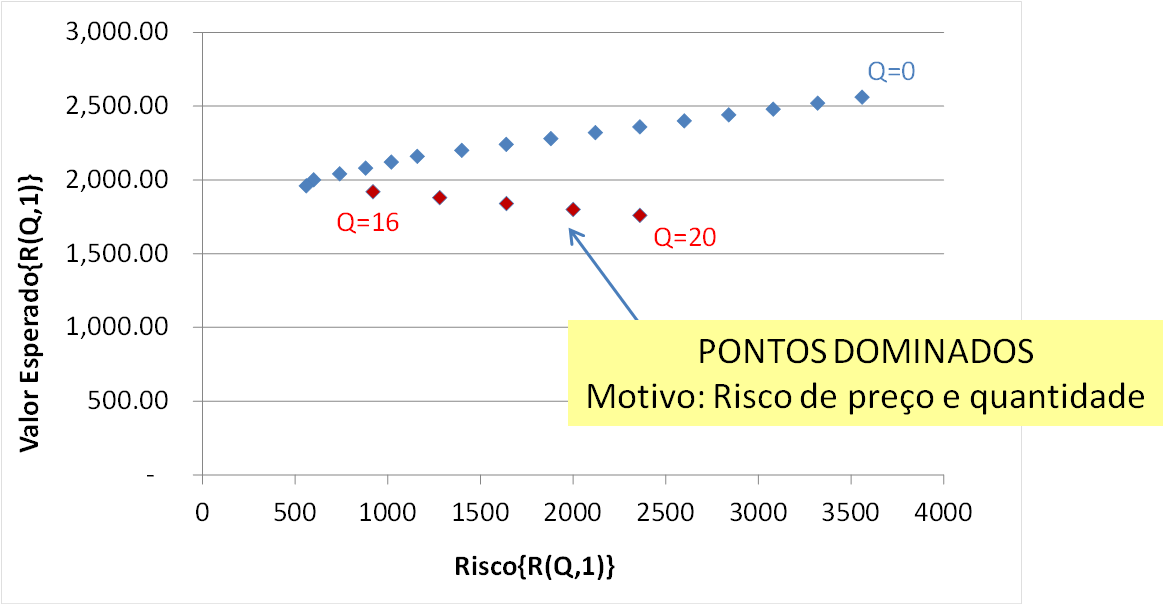
\includegraphics[scale=0.6]{aula10_49}\protect\caption{\label{fig:aula10_49} Pontos dominados contratação ótima}
\end{centering}
\end{figure}

\begin{figure}[H]
\begin{centering}
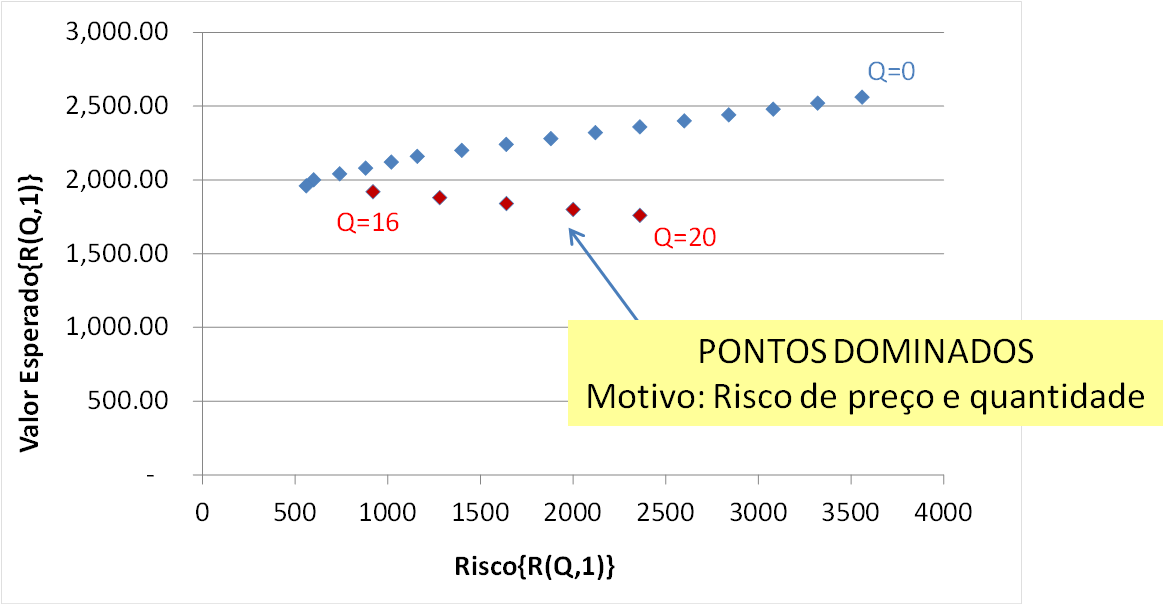
\includegraphics[scale=0.6]{aula10_49}\protect\caption{\label{fig:aula10_49} Pontos para $x=1$ dominam os demais pontos}
\end{centering}
\end{figure}

